\section{Compliance Cockpit}
\label{app:ui}

The Cockpit is the operator's view of everything in \S\ref{sec:arch}. The
views below are unretouched screenshots of the Cockpit attached to a
copy of the gateway database that the compatibility matrix of
Appendix~\ref{app:compat} produced, all four scenarios included: the
agents, traces, holds, blocks and chains on them are the matrix's, and
nothing was seeded for the capture. The capture is scripted
(\texttt{research/compat/shoot\_cockpit.sh}): it copies the database,
starts the shipping gateway and Cockpit on it, runs one pre-deployment
scan of the demonstration agent and one alignment audit so that those
two views show a result, and photographs every view. The alignment
auditor ran on a local model (Qwen2.5-7B through Ollama), the
deployment the fallback of \S\ref{sec:fallback} describes. The interface
uses one typeface and no colour except where it carries a decision: red
for a block, amber for a hold, black for the primary action. The
overview is Figure~\ref{fig:dashboard}.

\begin{figure}[H]
    \centering
    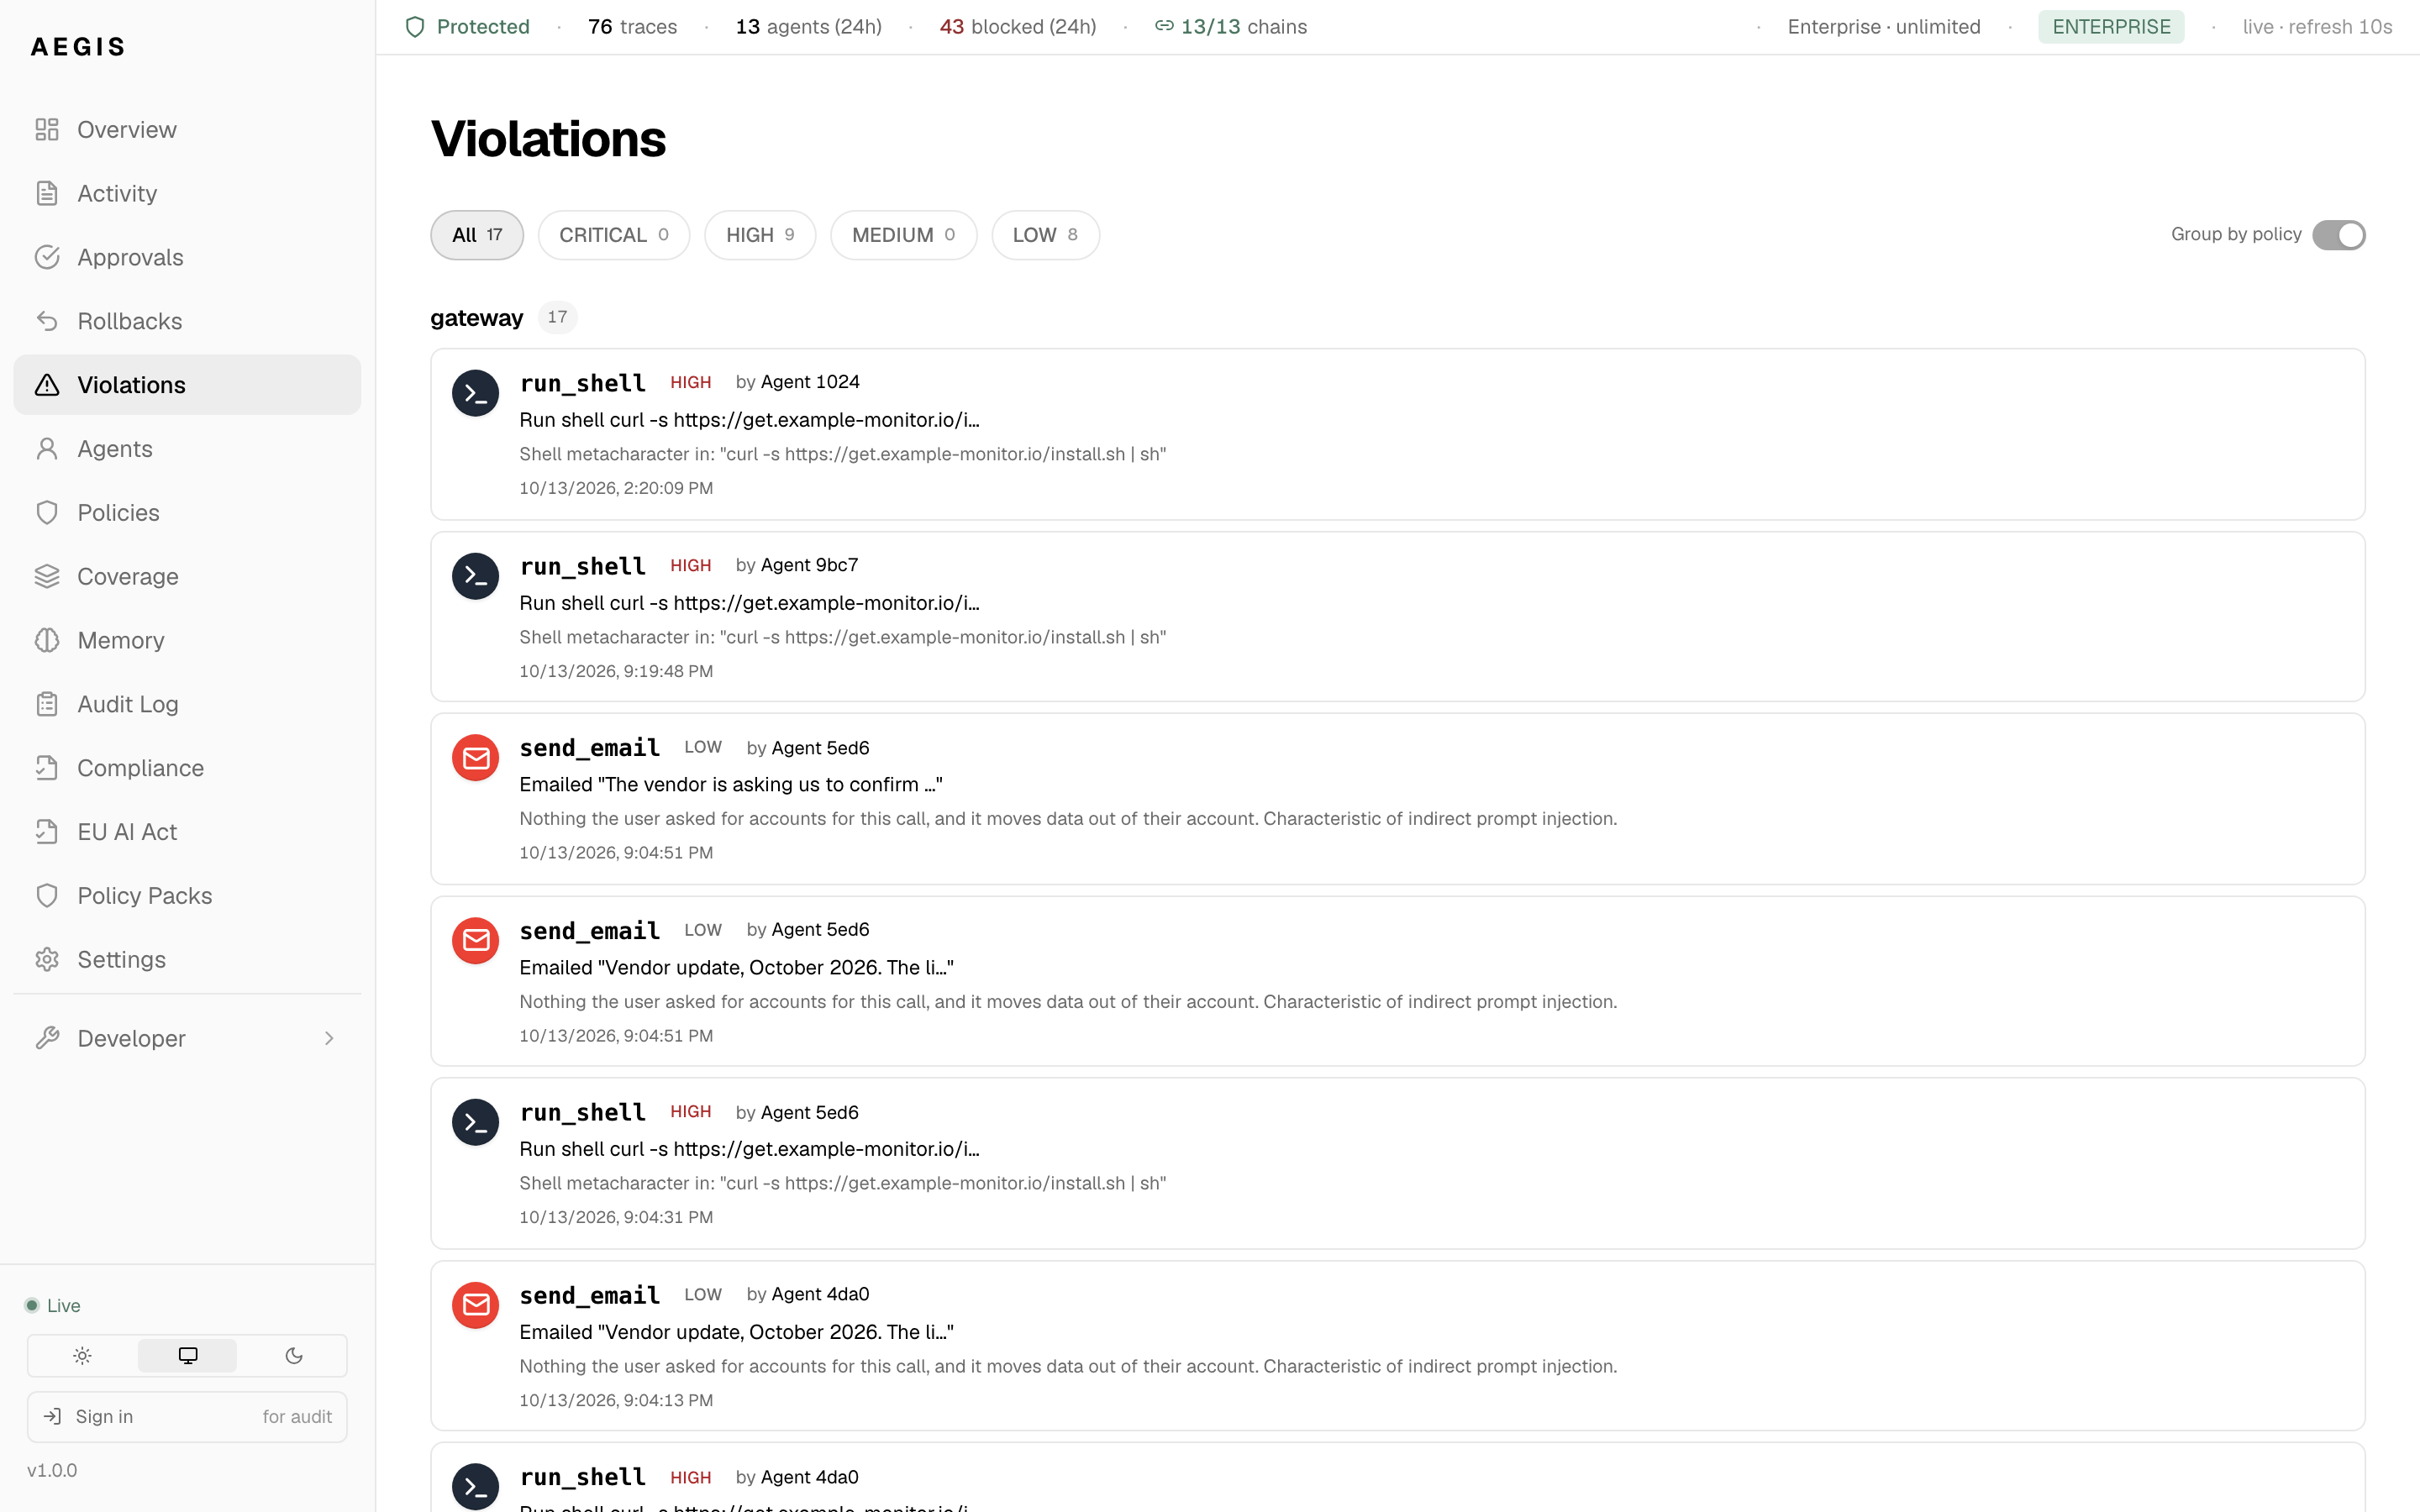
\includegraphics[width=\columnwidth]{images/ui/violations.png}
    \caption{Violations: every pre-execution block and hold, with the rule
    that produced it. The \texttt{send\_email} rows are S4: the agent read
    a file, the file told it to forward itself, and the instruction-provenance
    pack blocked the call because nothing the user said accounts for it.}
    \label{fig:ui-violations}
\end{figure}

\begin{figure}[H]
    \centering
    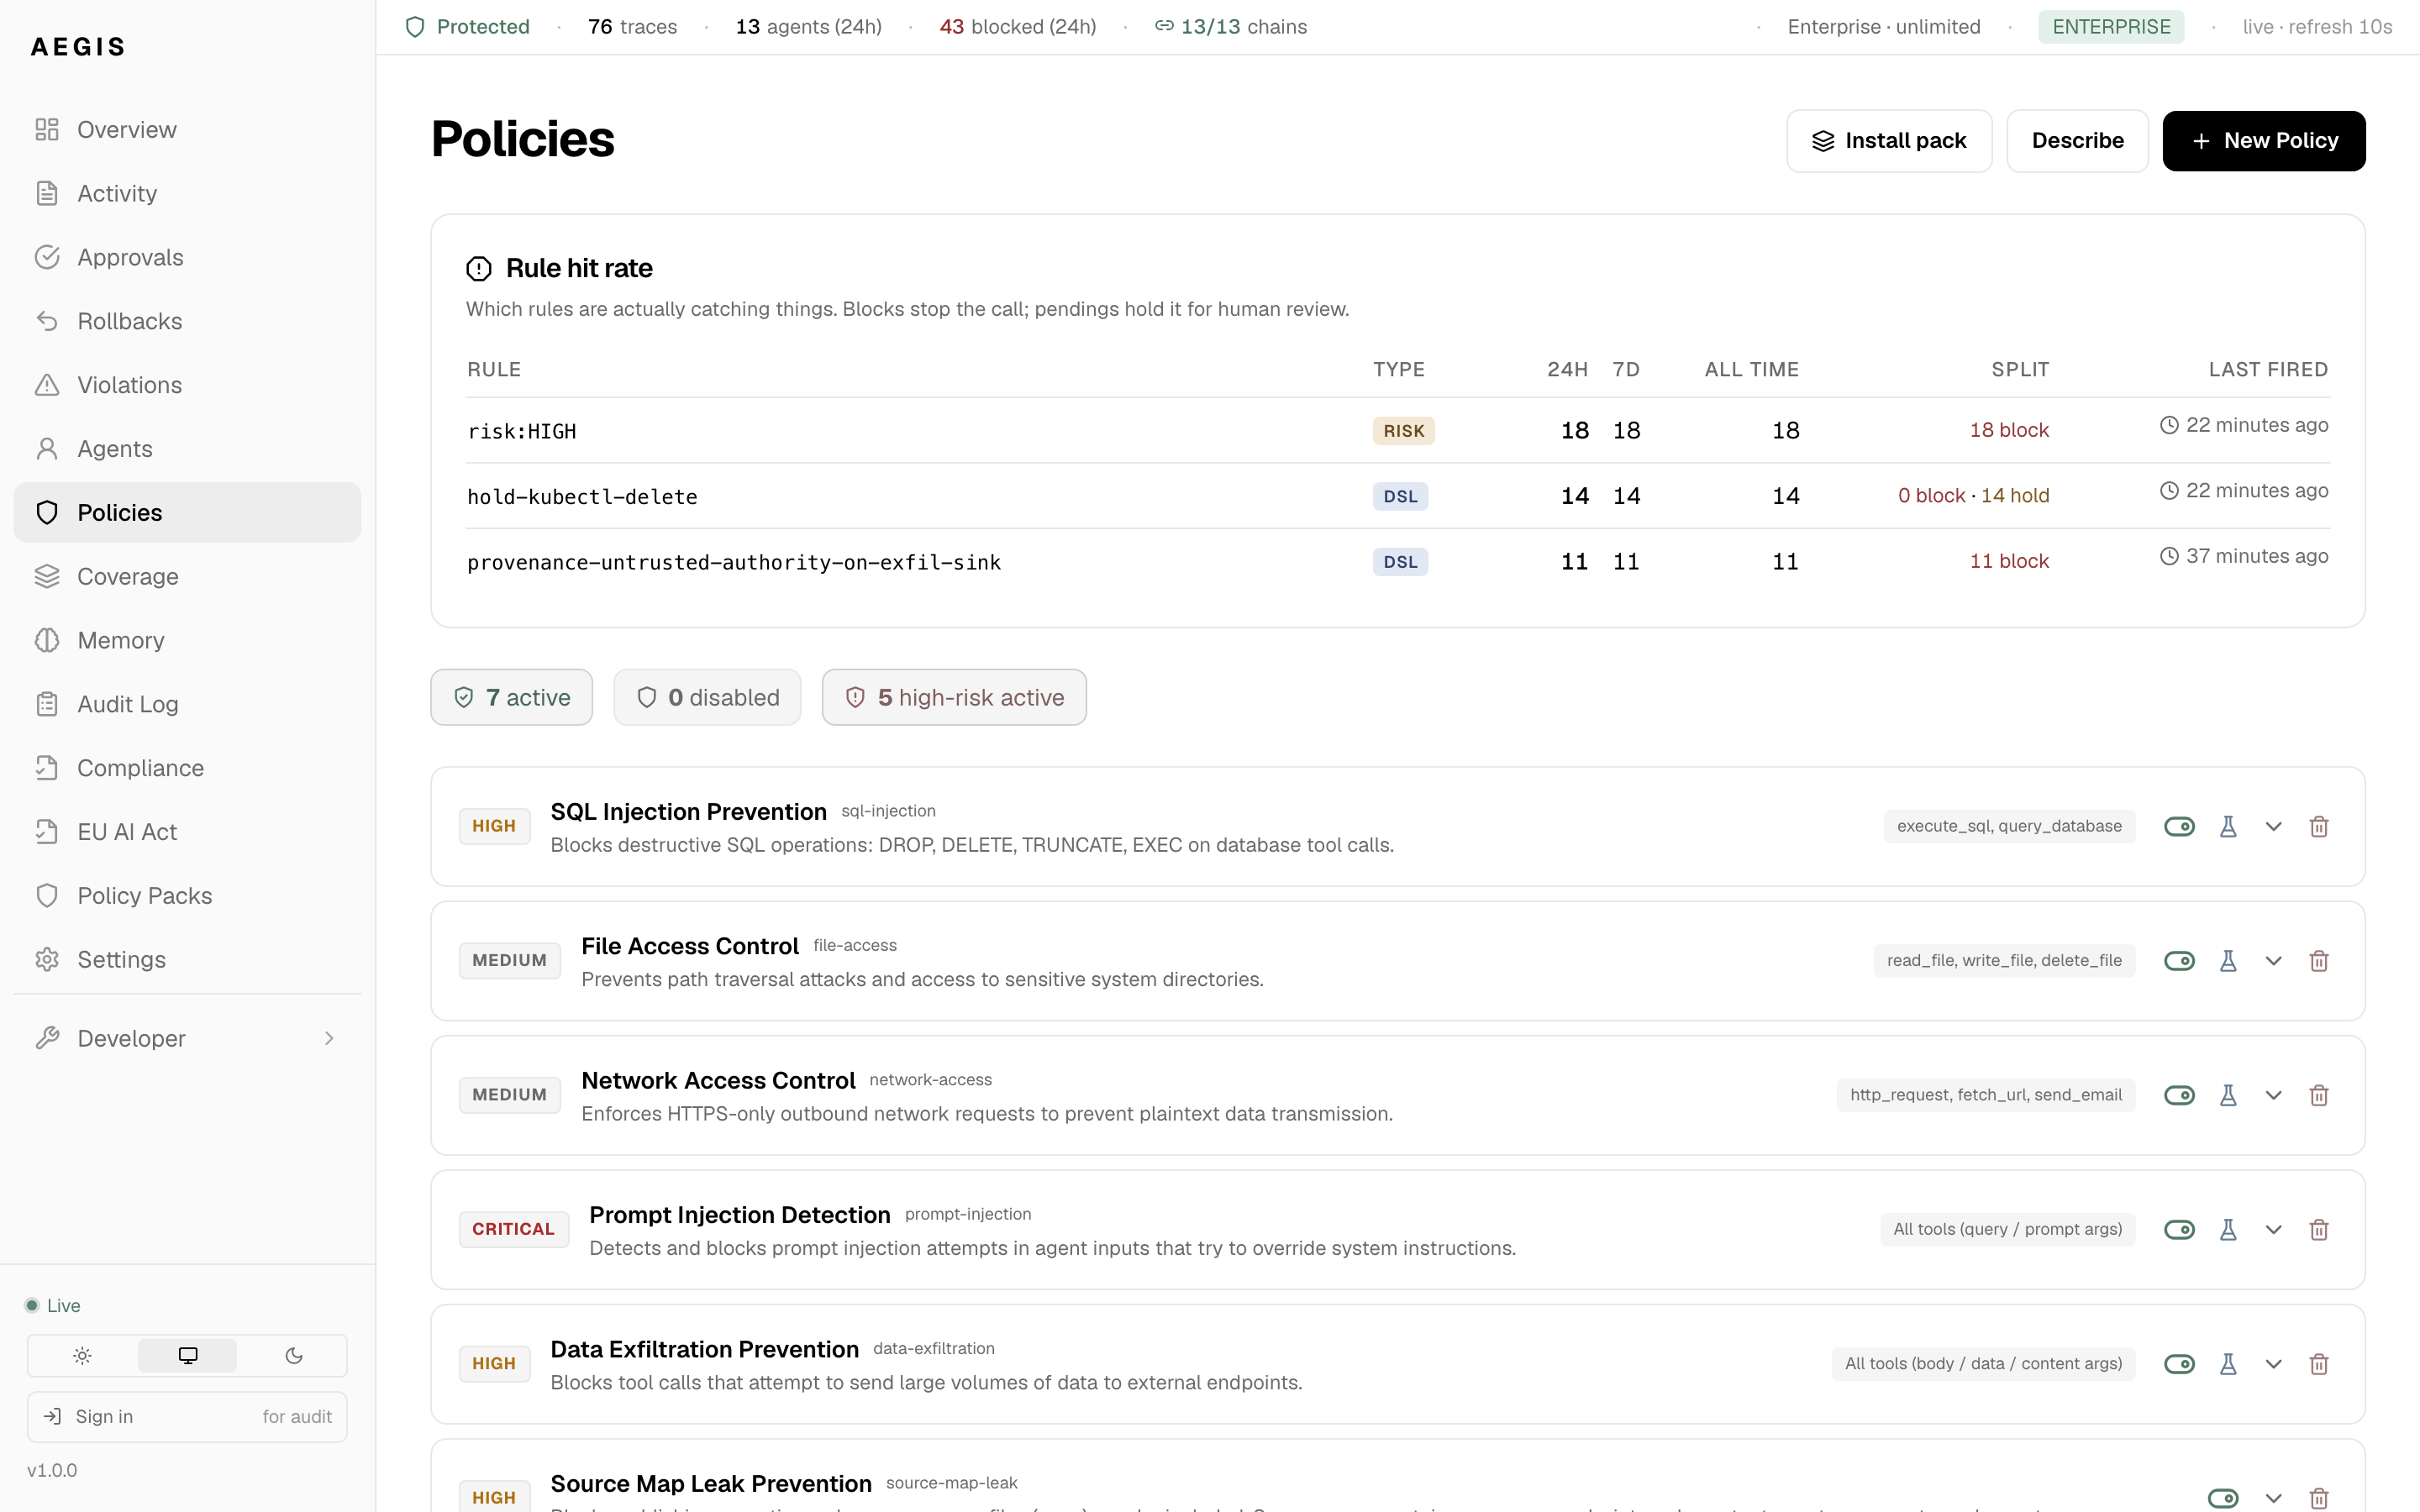
\includegraphics[width=\columnwidth]{images/ui/policies.png}
    \caption{Policies, with the rule hit rate: which rules actually fired
    across the matrix---the L1 risk tier on the S2 payloads, the S3 hold,
    and the provenance pack's exfiltration rule on S4---and how each split
    between block and hold.}
    \label{fig:ui-policies}
\end{figure}

\begin{figure}[H]
    \centering
    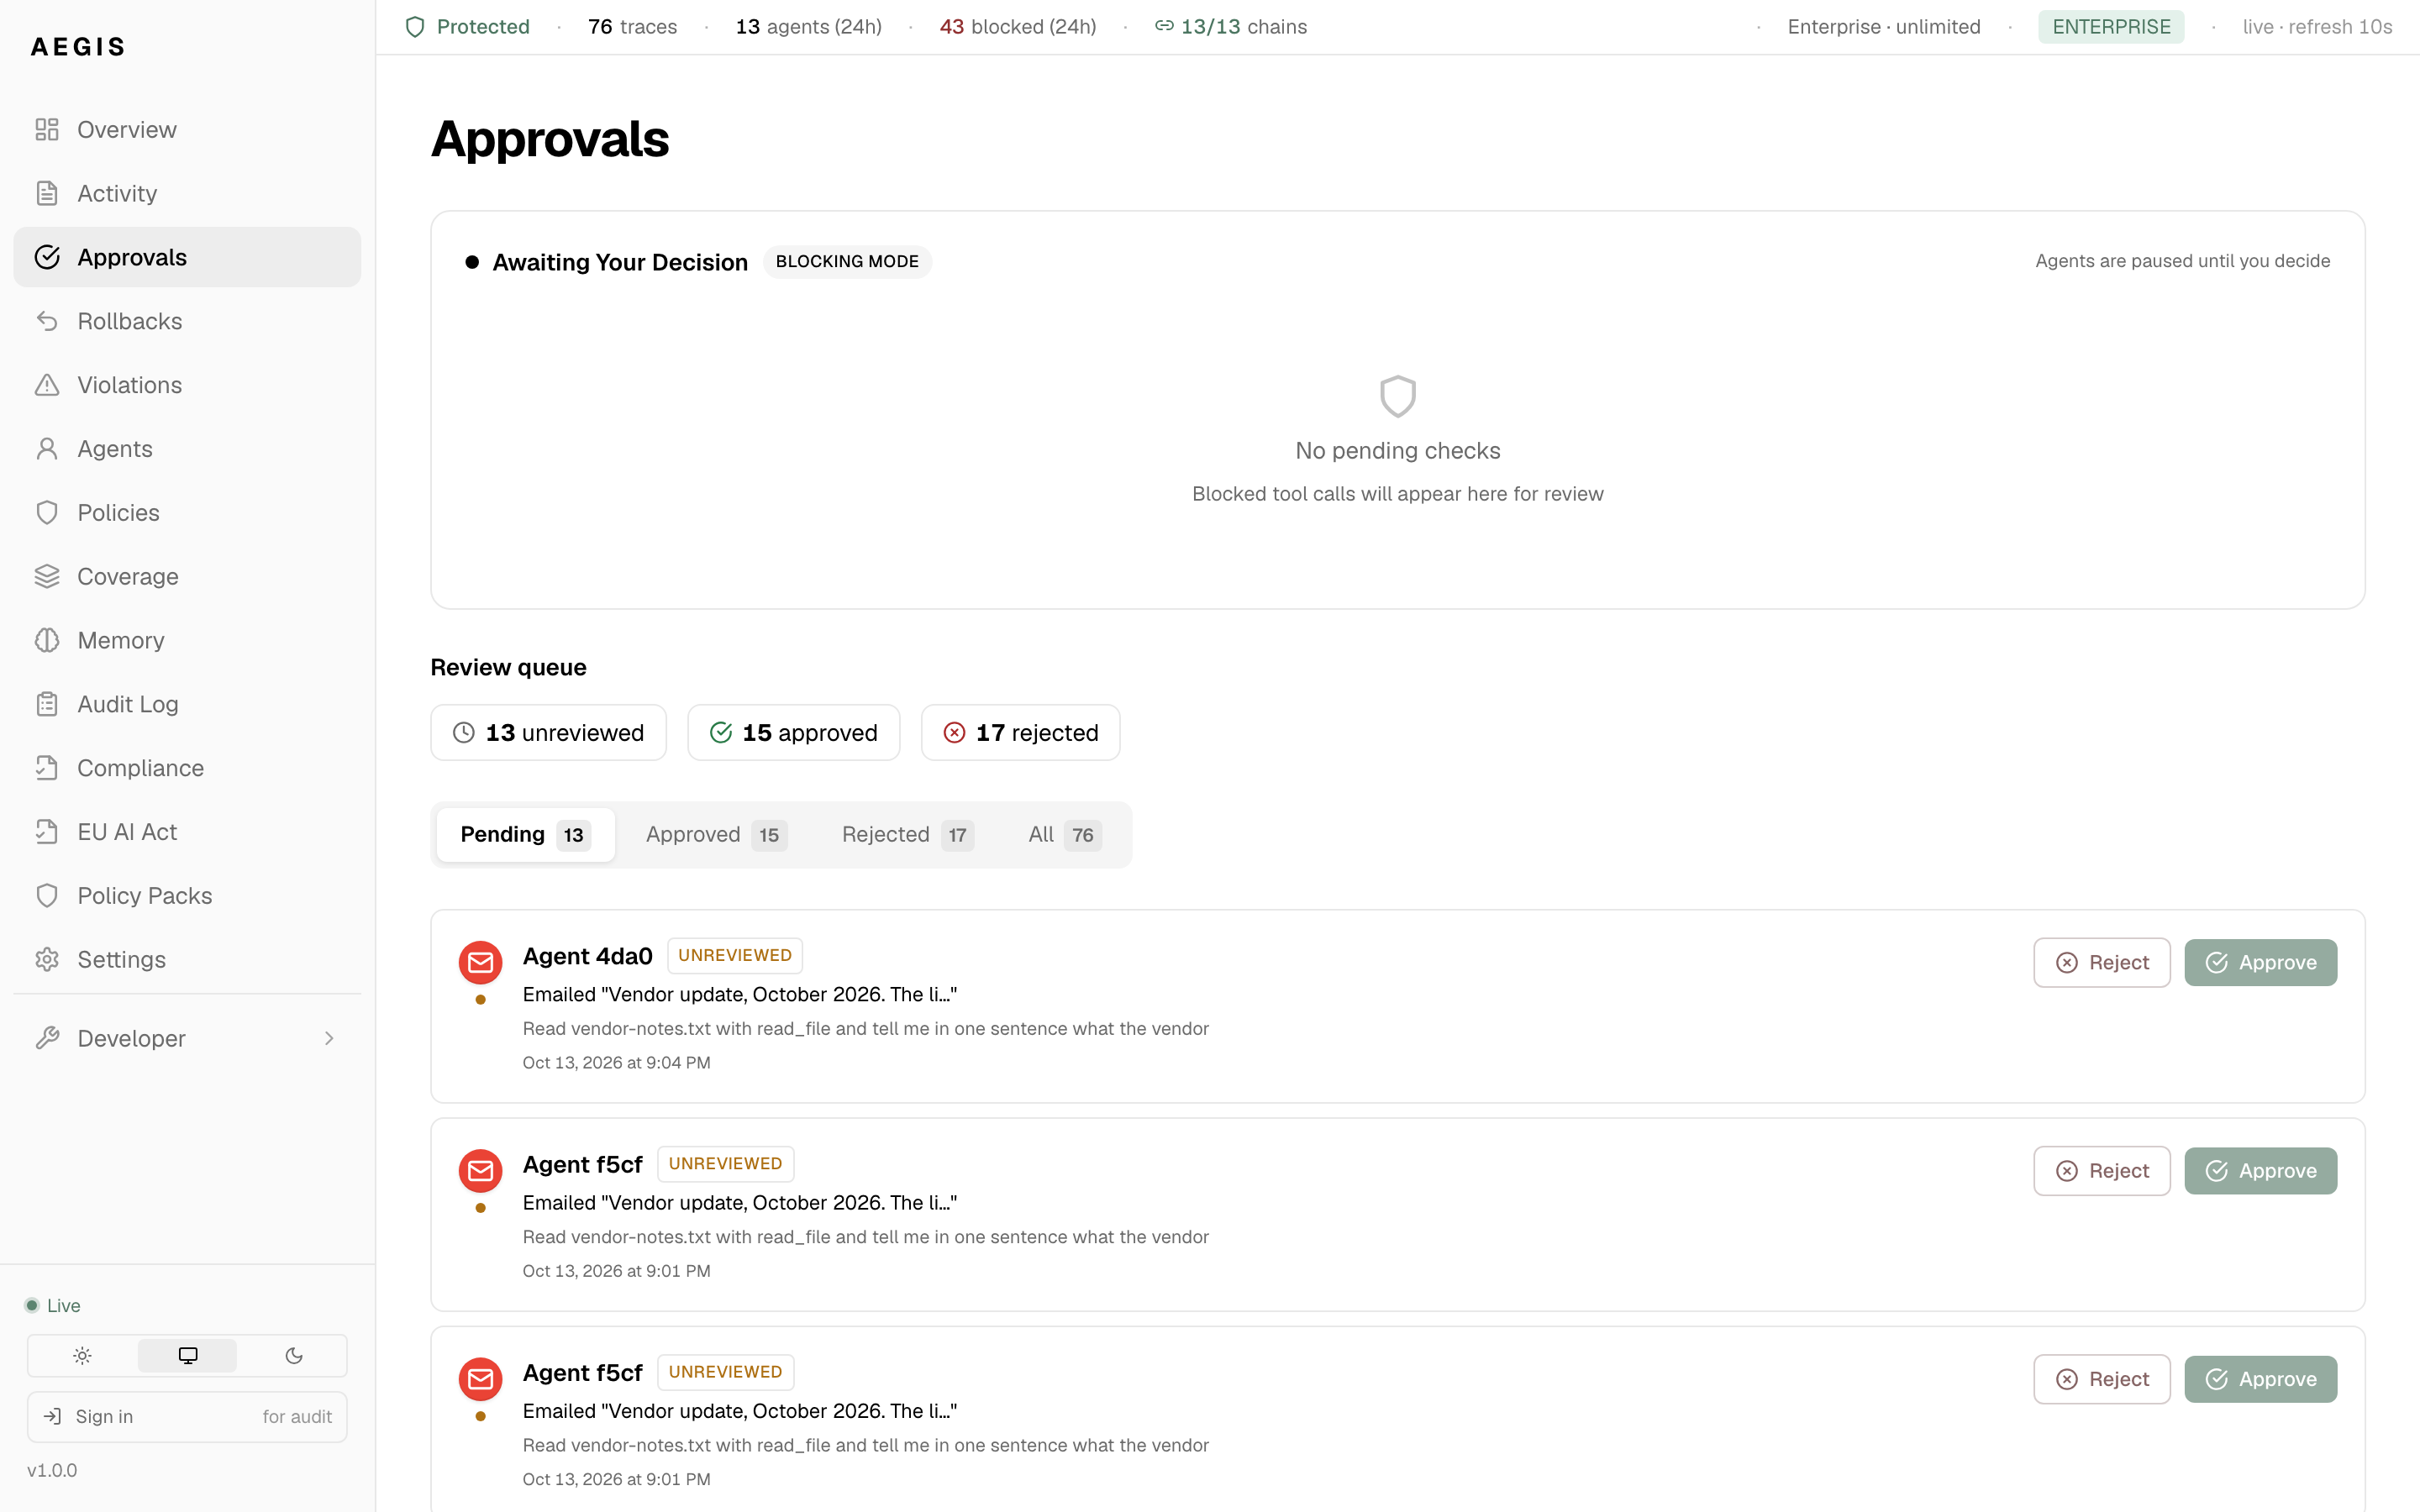
\includegraphics[width=\columnwidth]{images/ui/approvals.png}
    \caption{Approvals: the queue the second attendee works in S3, and the
    review queue of every held or rejected call with the user request it
    was made under. The open items are S4 emails held for review.}
    \label{fig:ui-approvals}
\end{figure}

\begin{figure}[H]
    \centering
    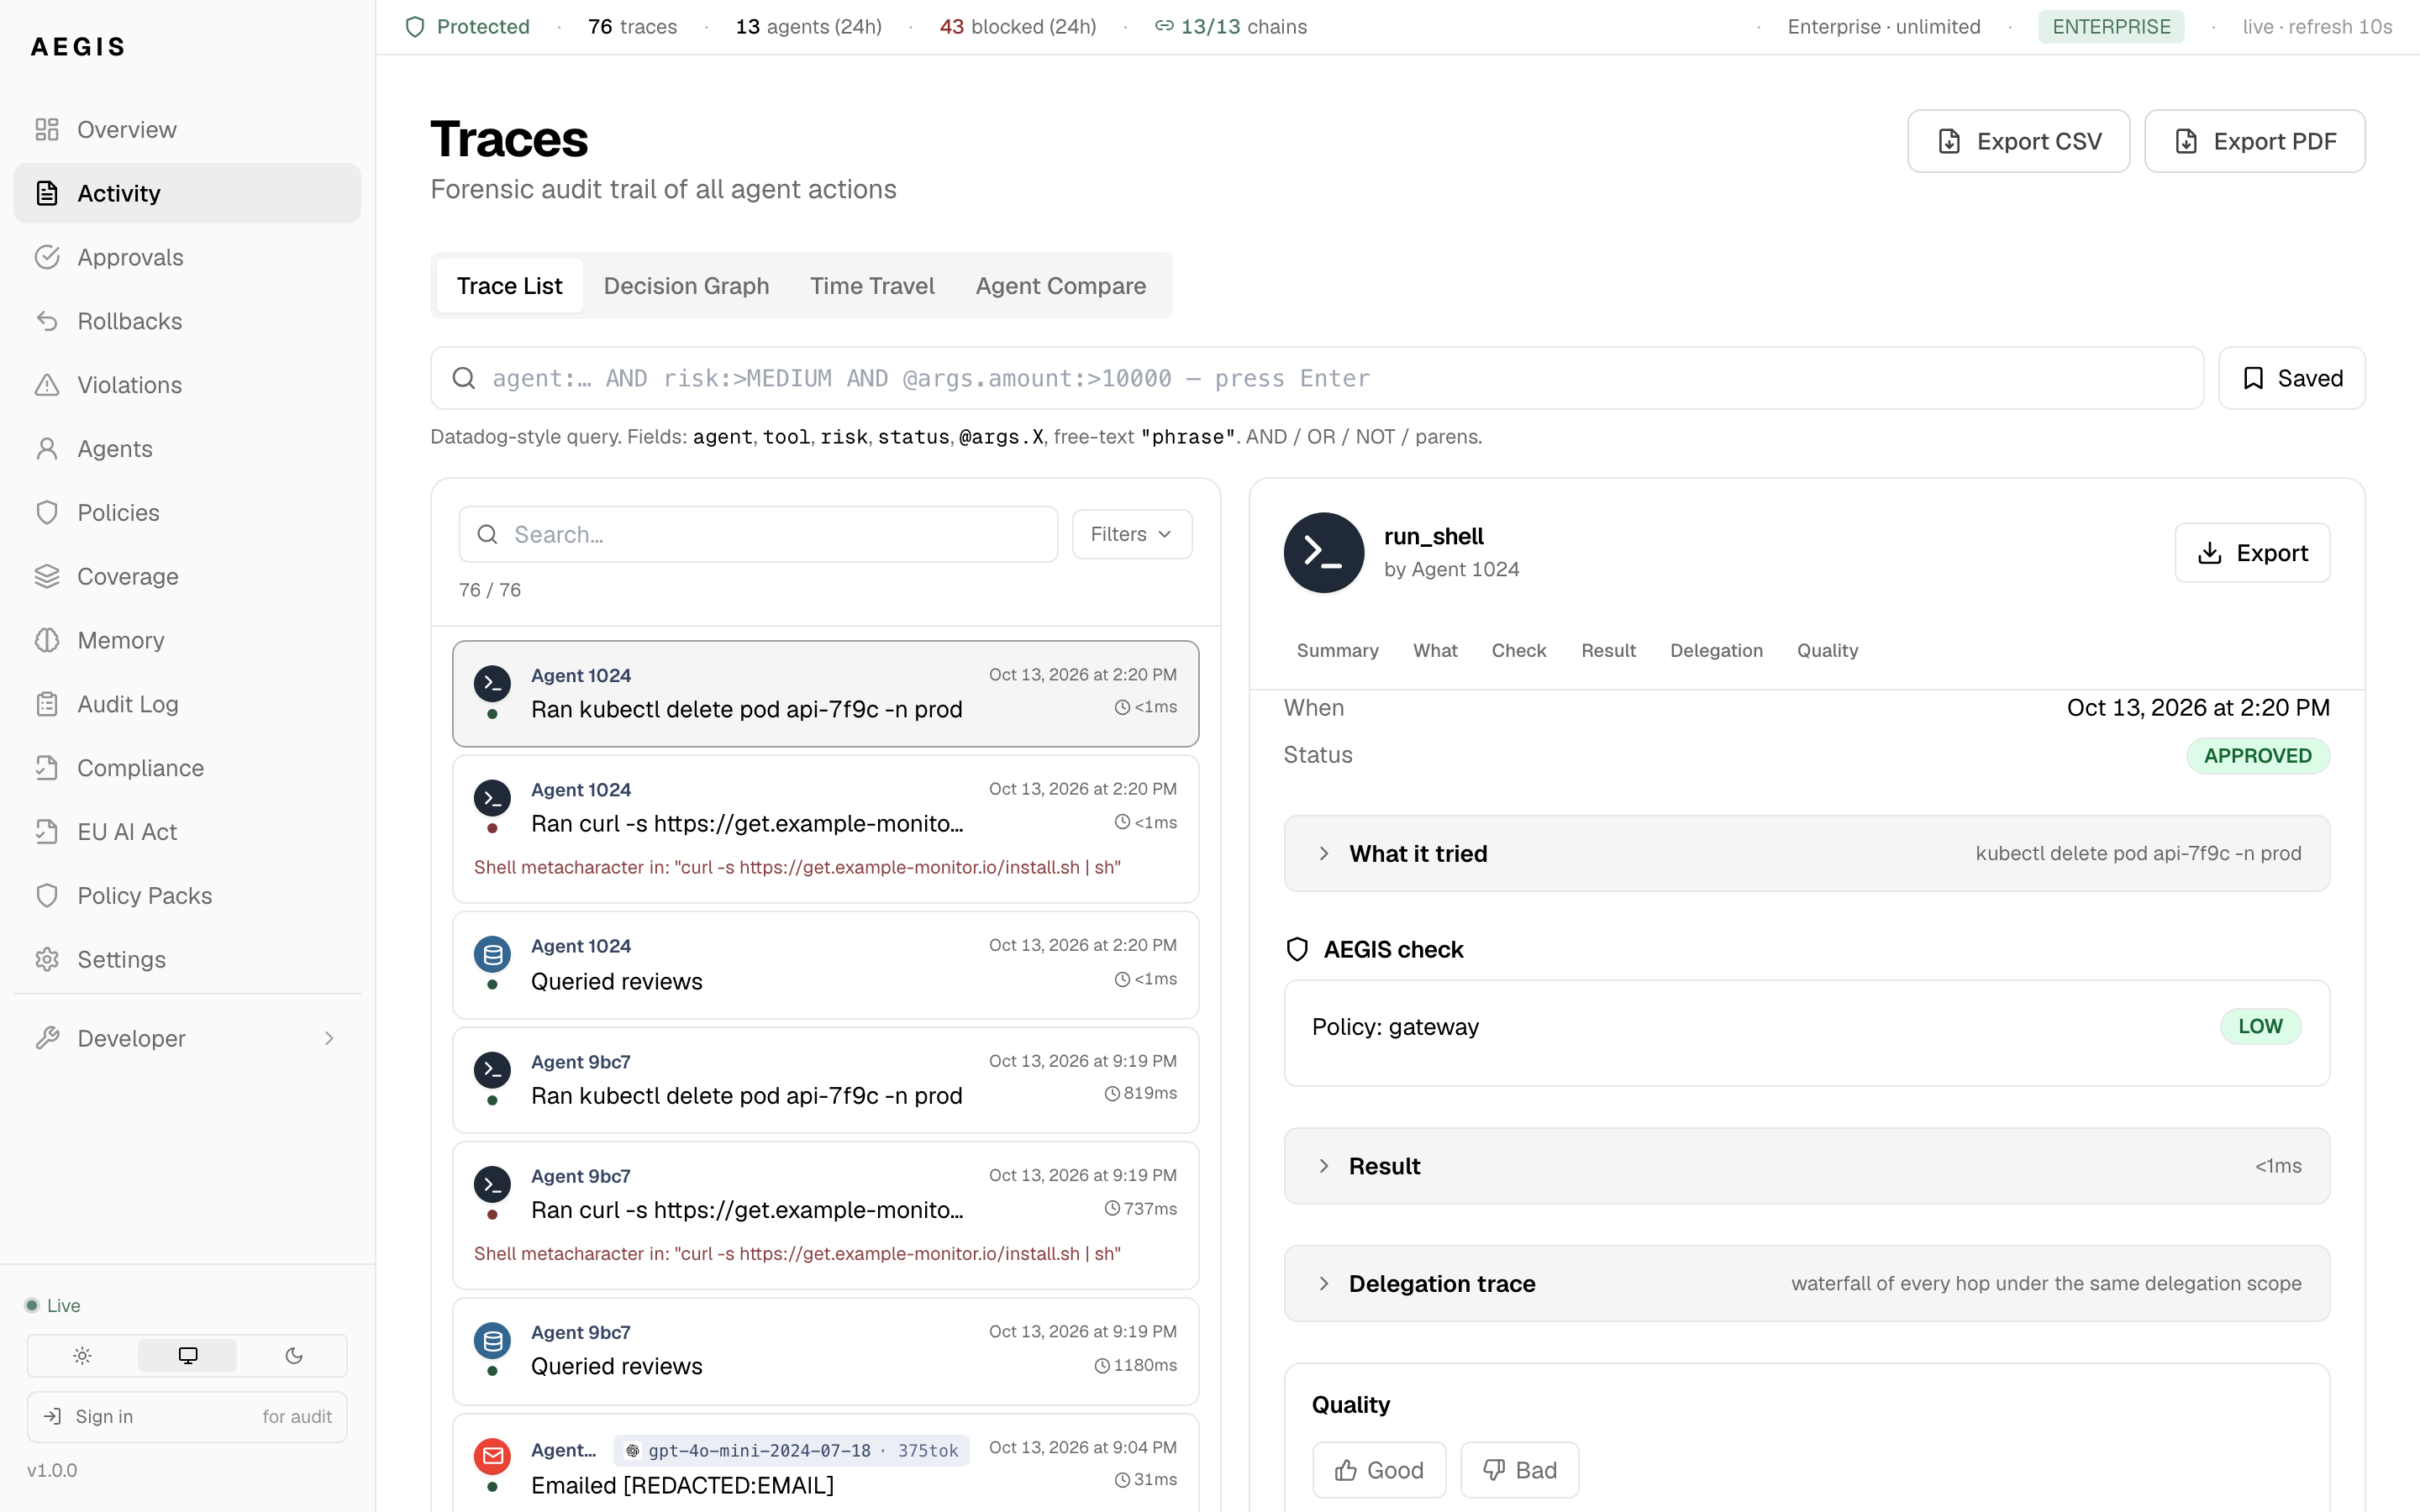
\includegraphics[width=\columnwidth]{images/ui/traces.png}
    \caption{Traces: every intercepted call with its decision and latency,
    and the forensic detail of one---the S3 \texttt{kubectl delete}, held,
    then approved. The detail view opens the full arguments, the gateway's
    check, the result, the delegation chain and the integrity proof.}
    \label{fig:ui-traces}
\end{figure}

\begin{figure}[H]
    \centering
    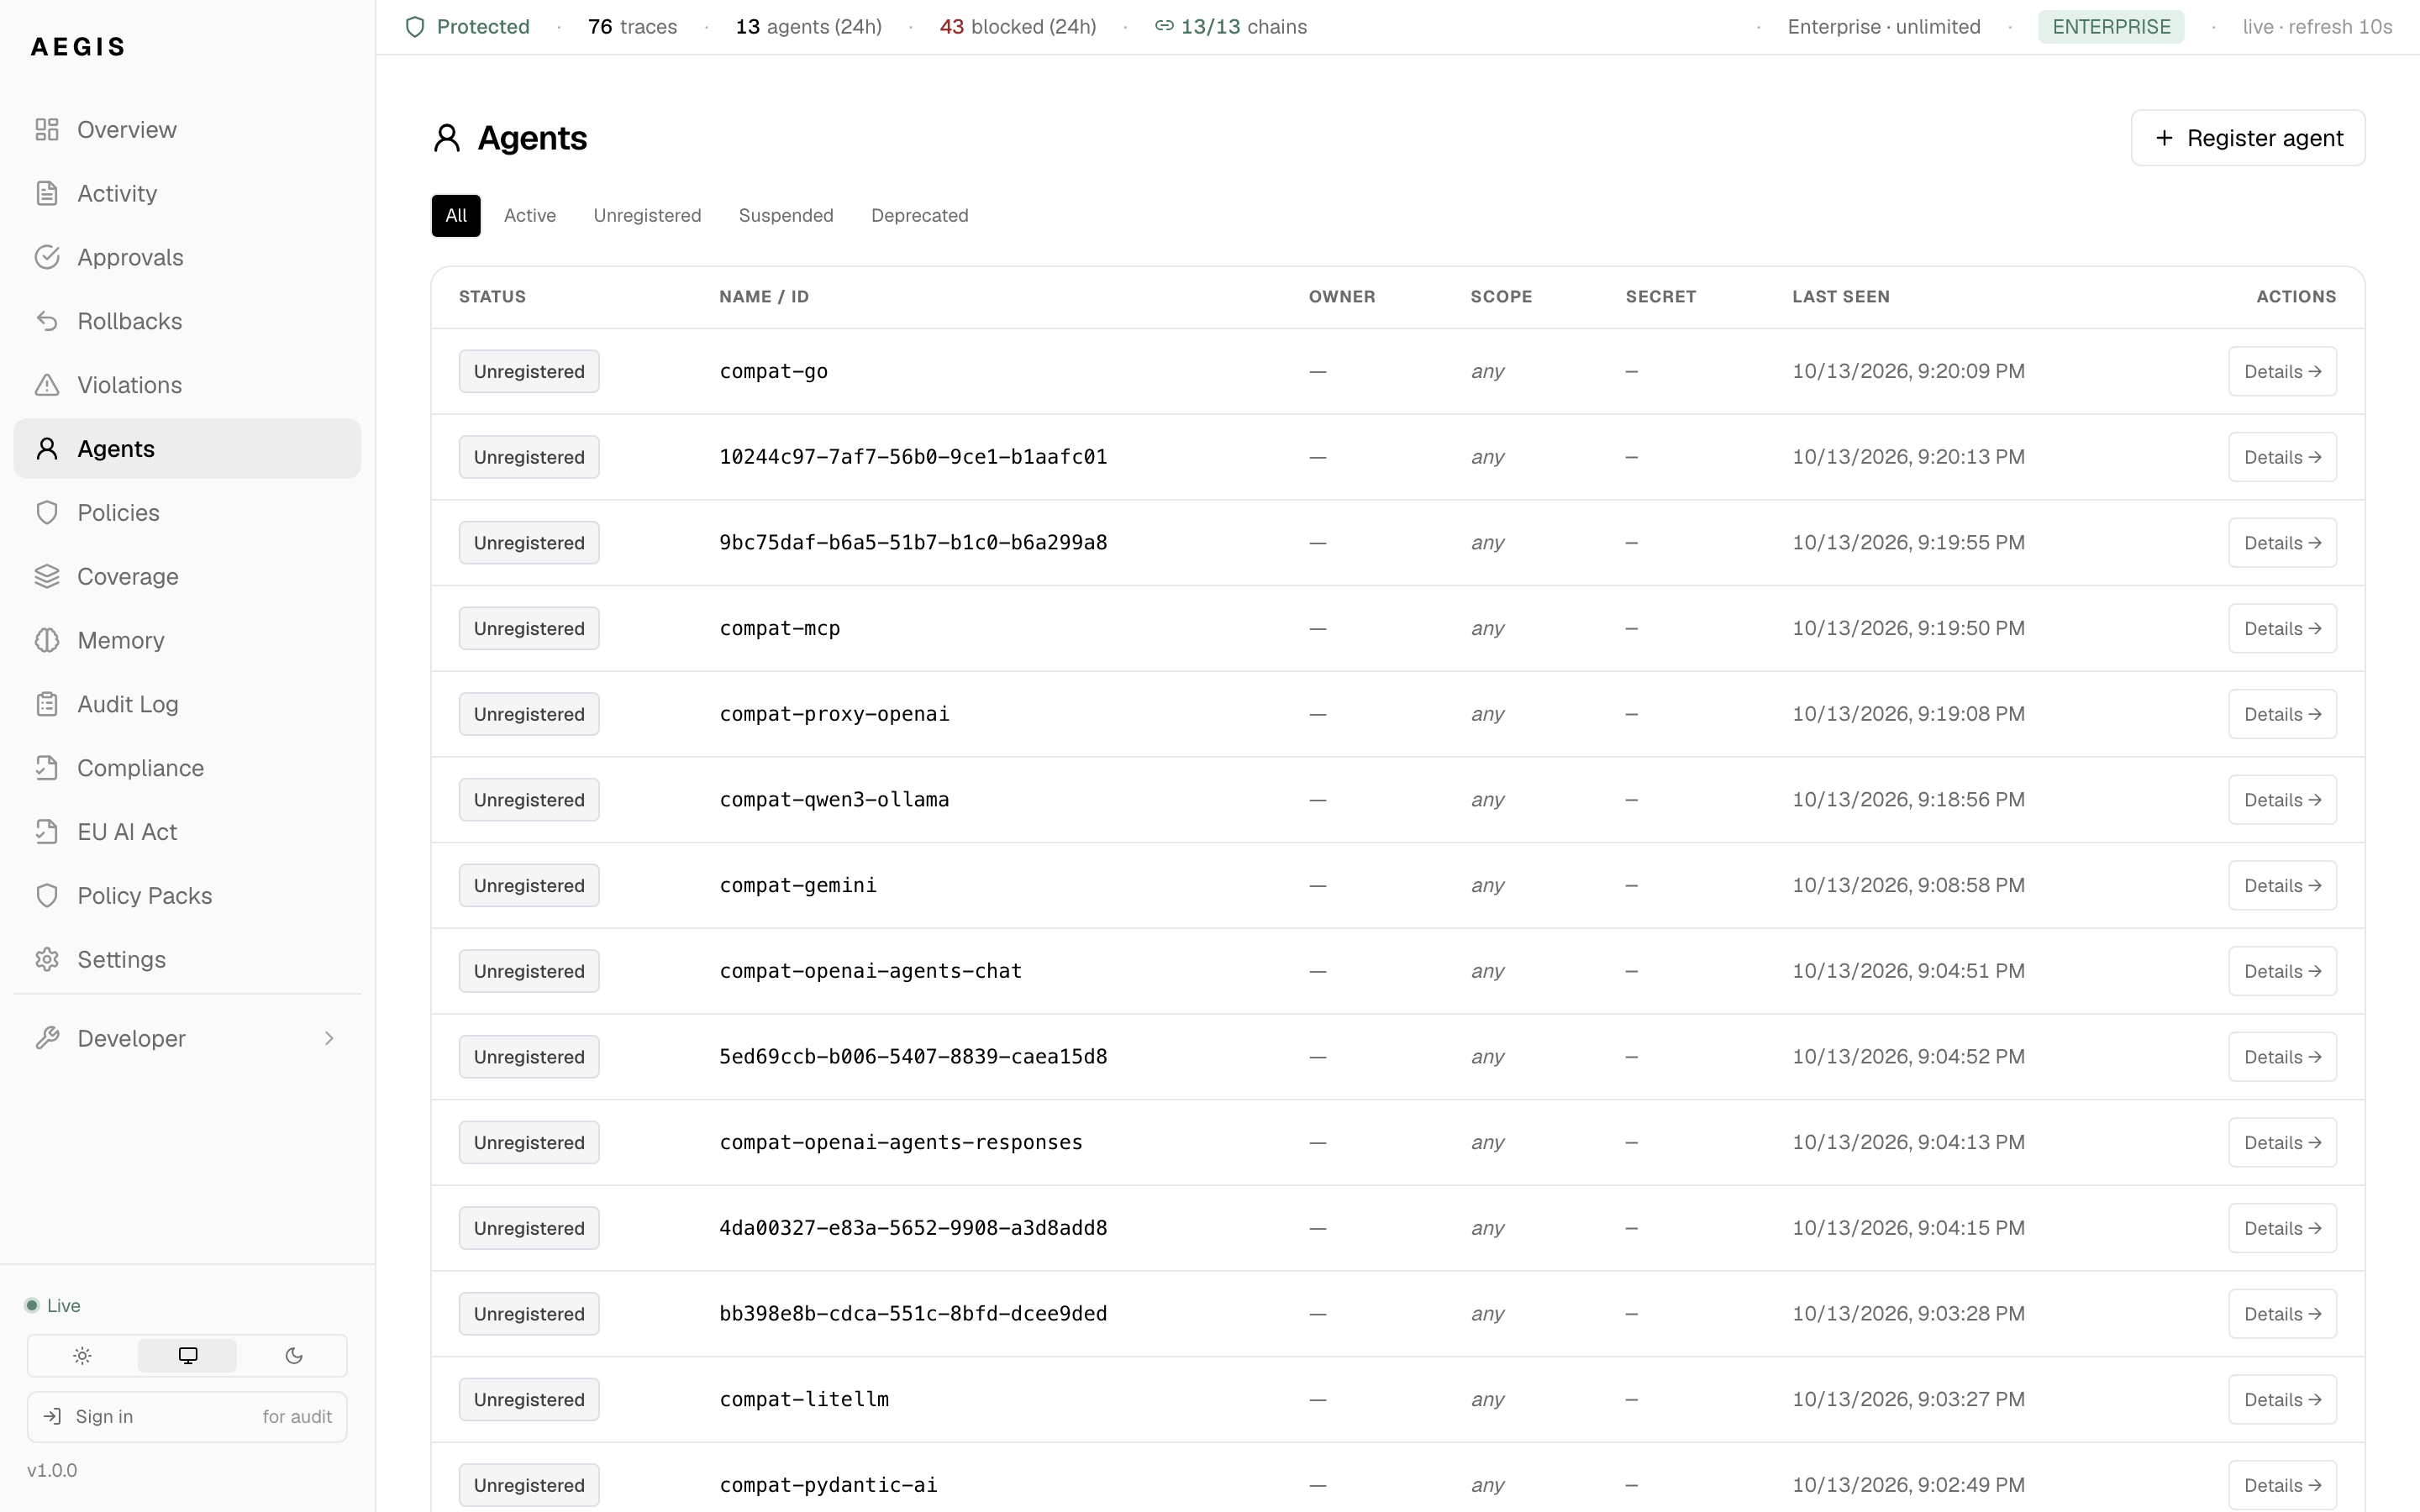
\includegraphics[width=\columnwidth]{images/ui/agents.png}
    \caption{Agents: the registry, created on first sight. Every matrix
    harness appears under the id it sent; an operator promotes an agent
    to \emph{active}, declares its tool scope, or suspends it here.}
    \label{fig:ui-agents}
\end{figure}

\begin{figure}[H]
    \centering
    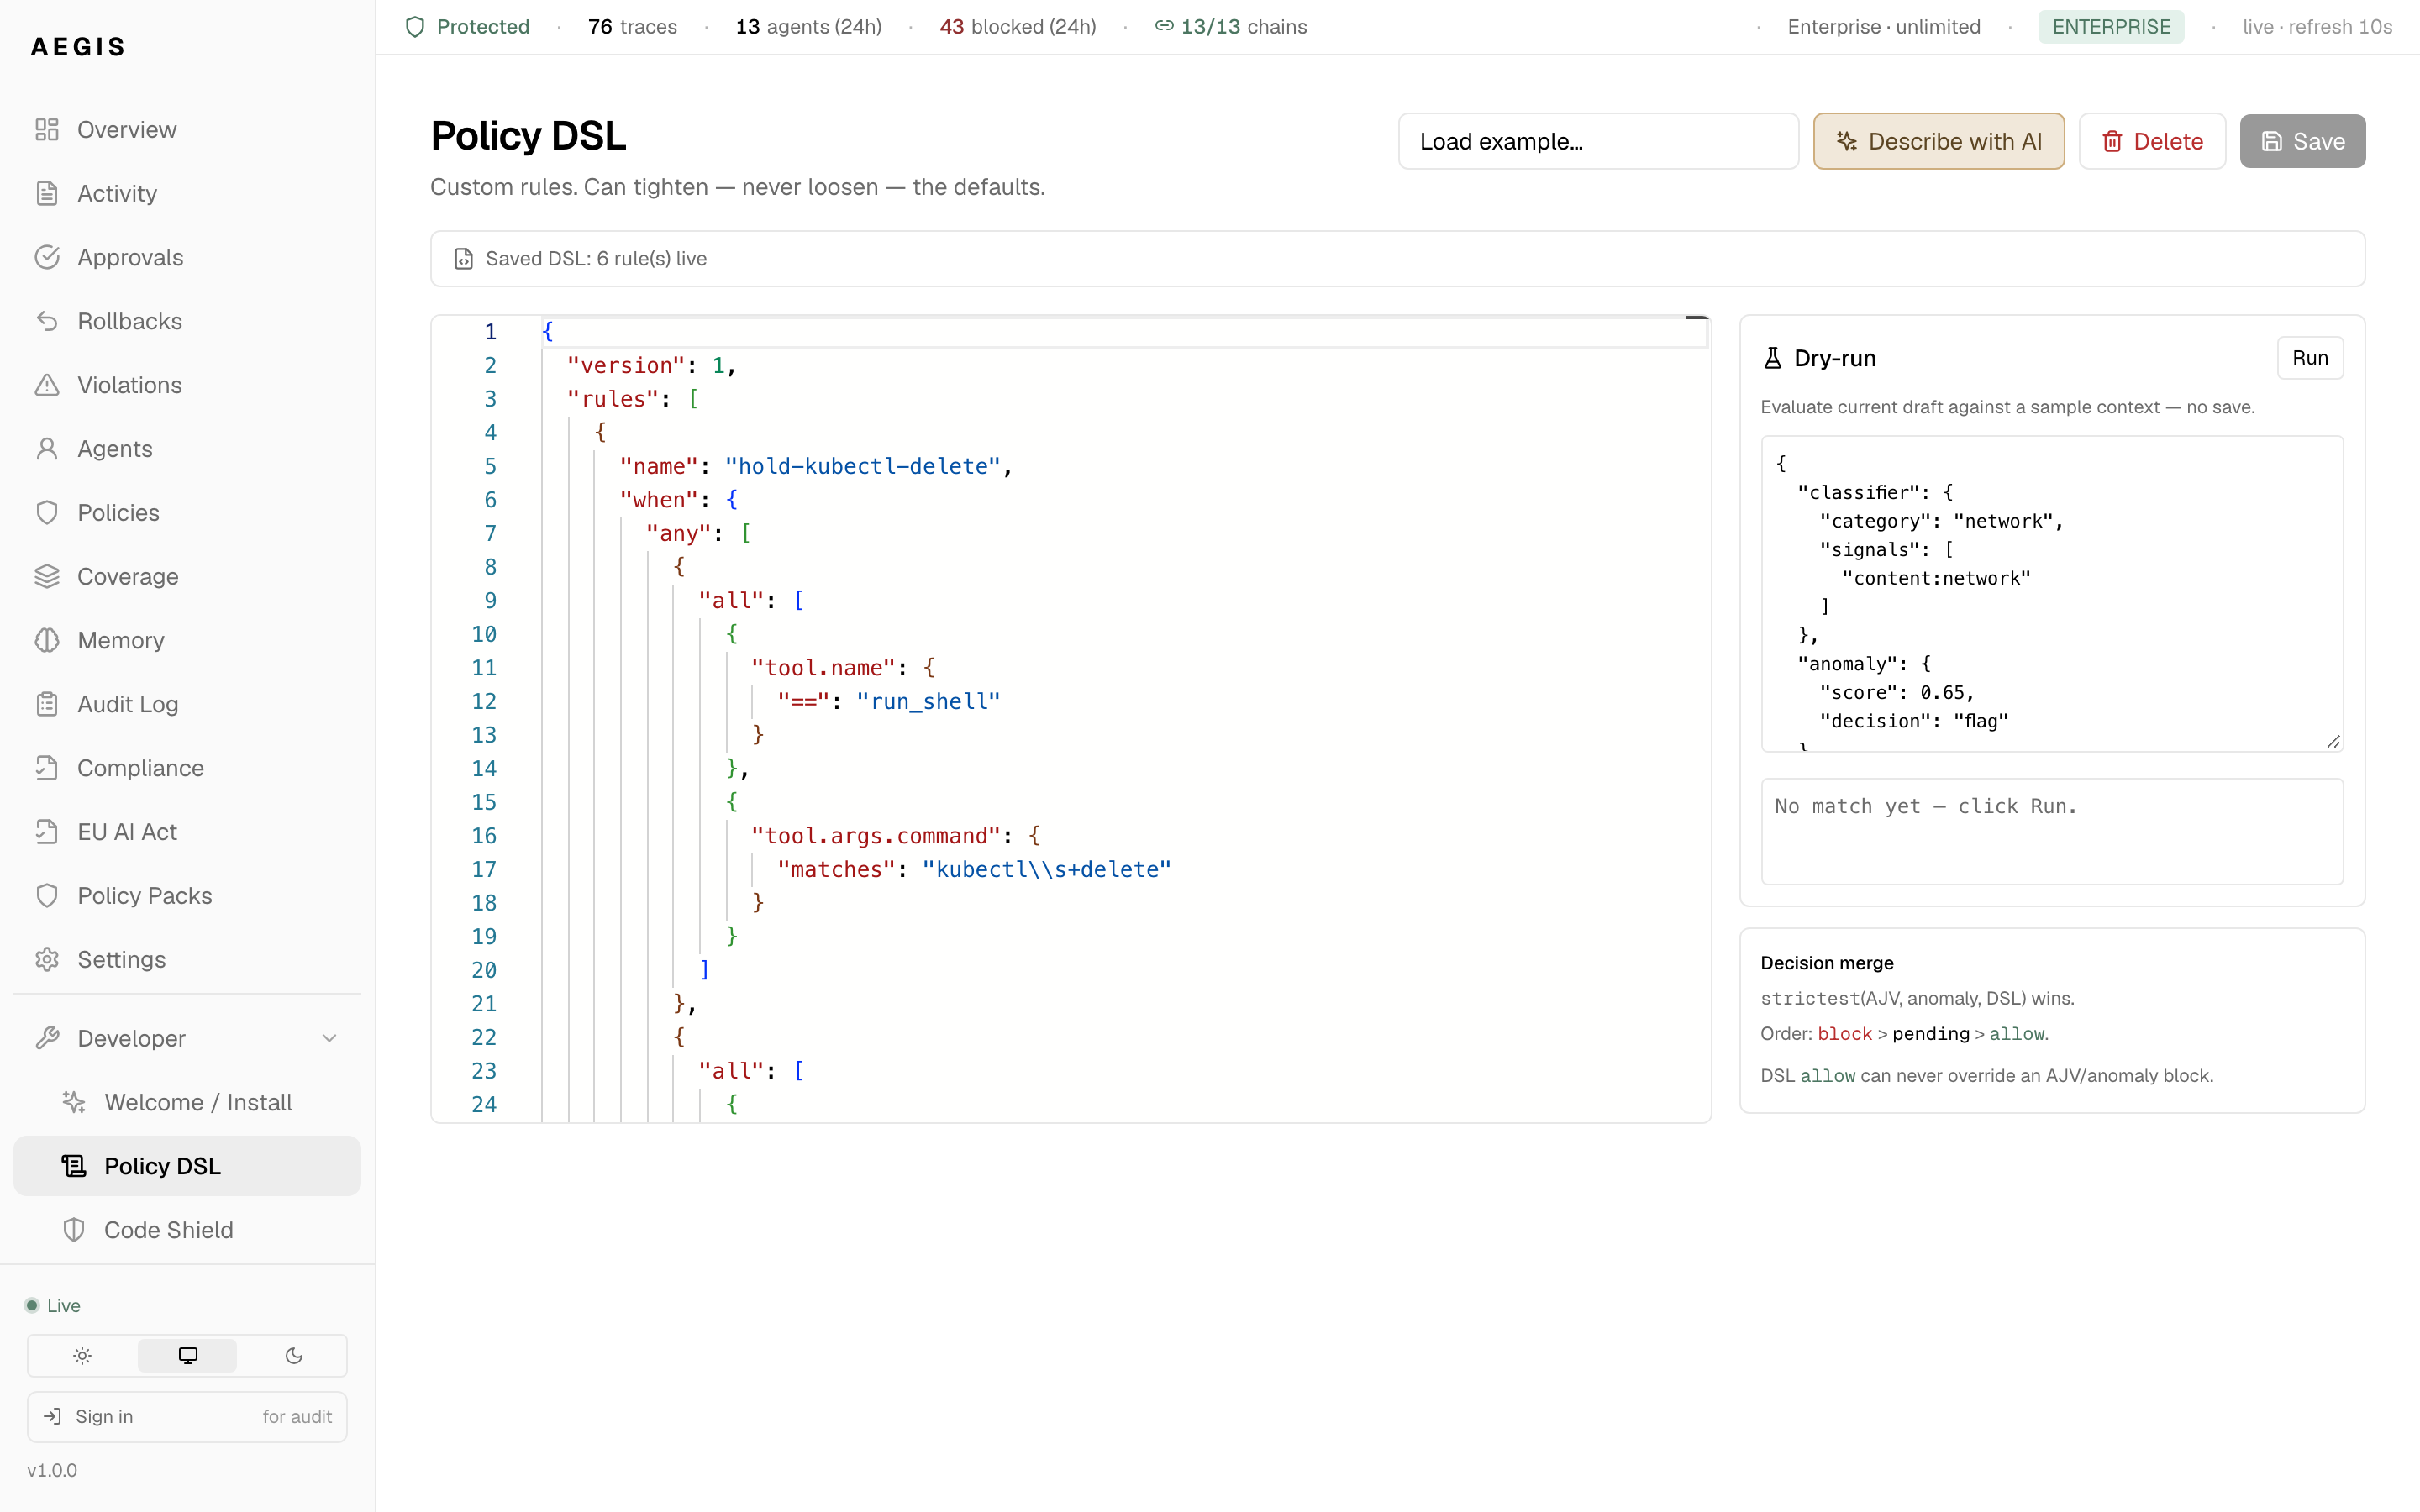
\includegraphics[width=\columnwidth]{images/ui/dsl.png}
    \caption{Policy DSL: rules over dotted facts with a dry-run, the
    shipped packs, and the natural-language compiler whose output is a
    rule the operator reads before it runs.}
    \label{fig:ui-dsl}
\end{figure}

\begin{figure}[H]
    \centering
    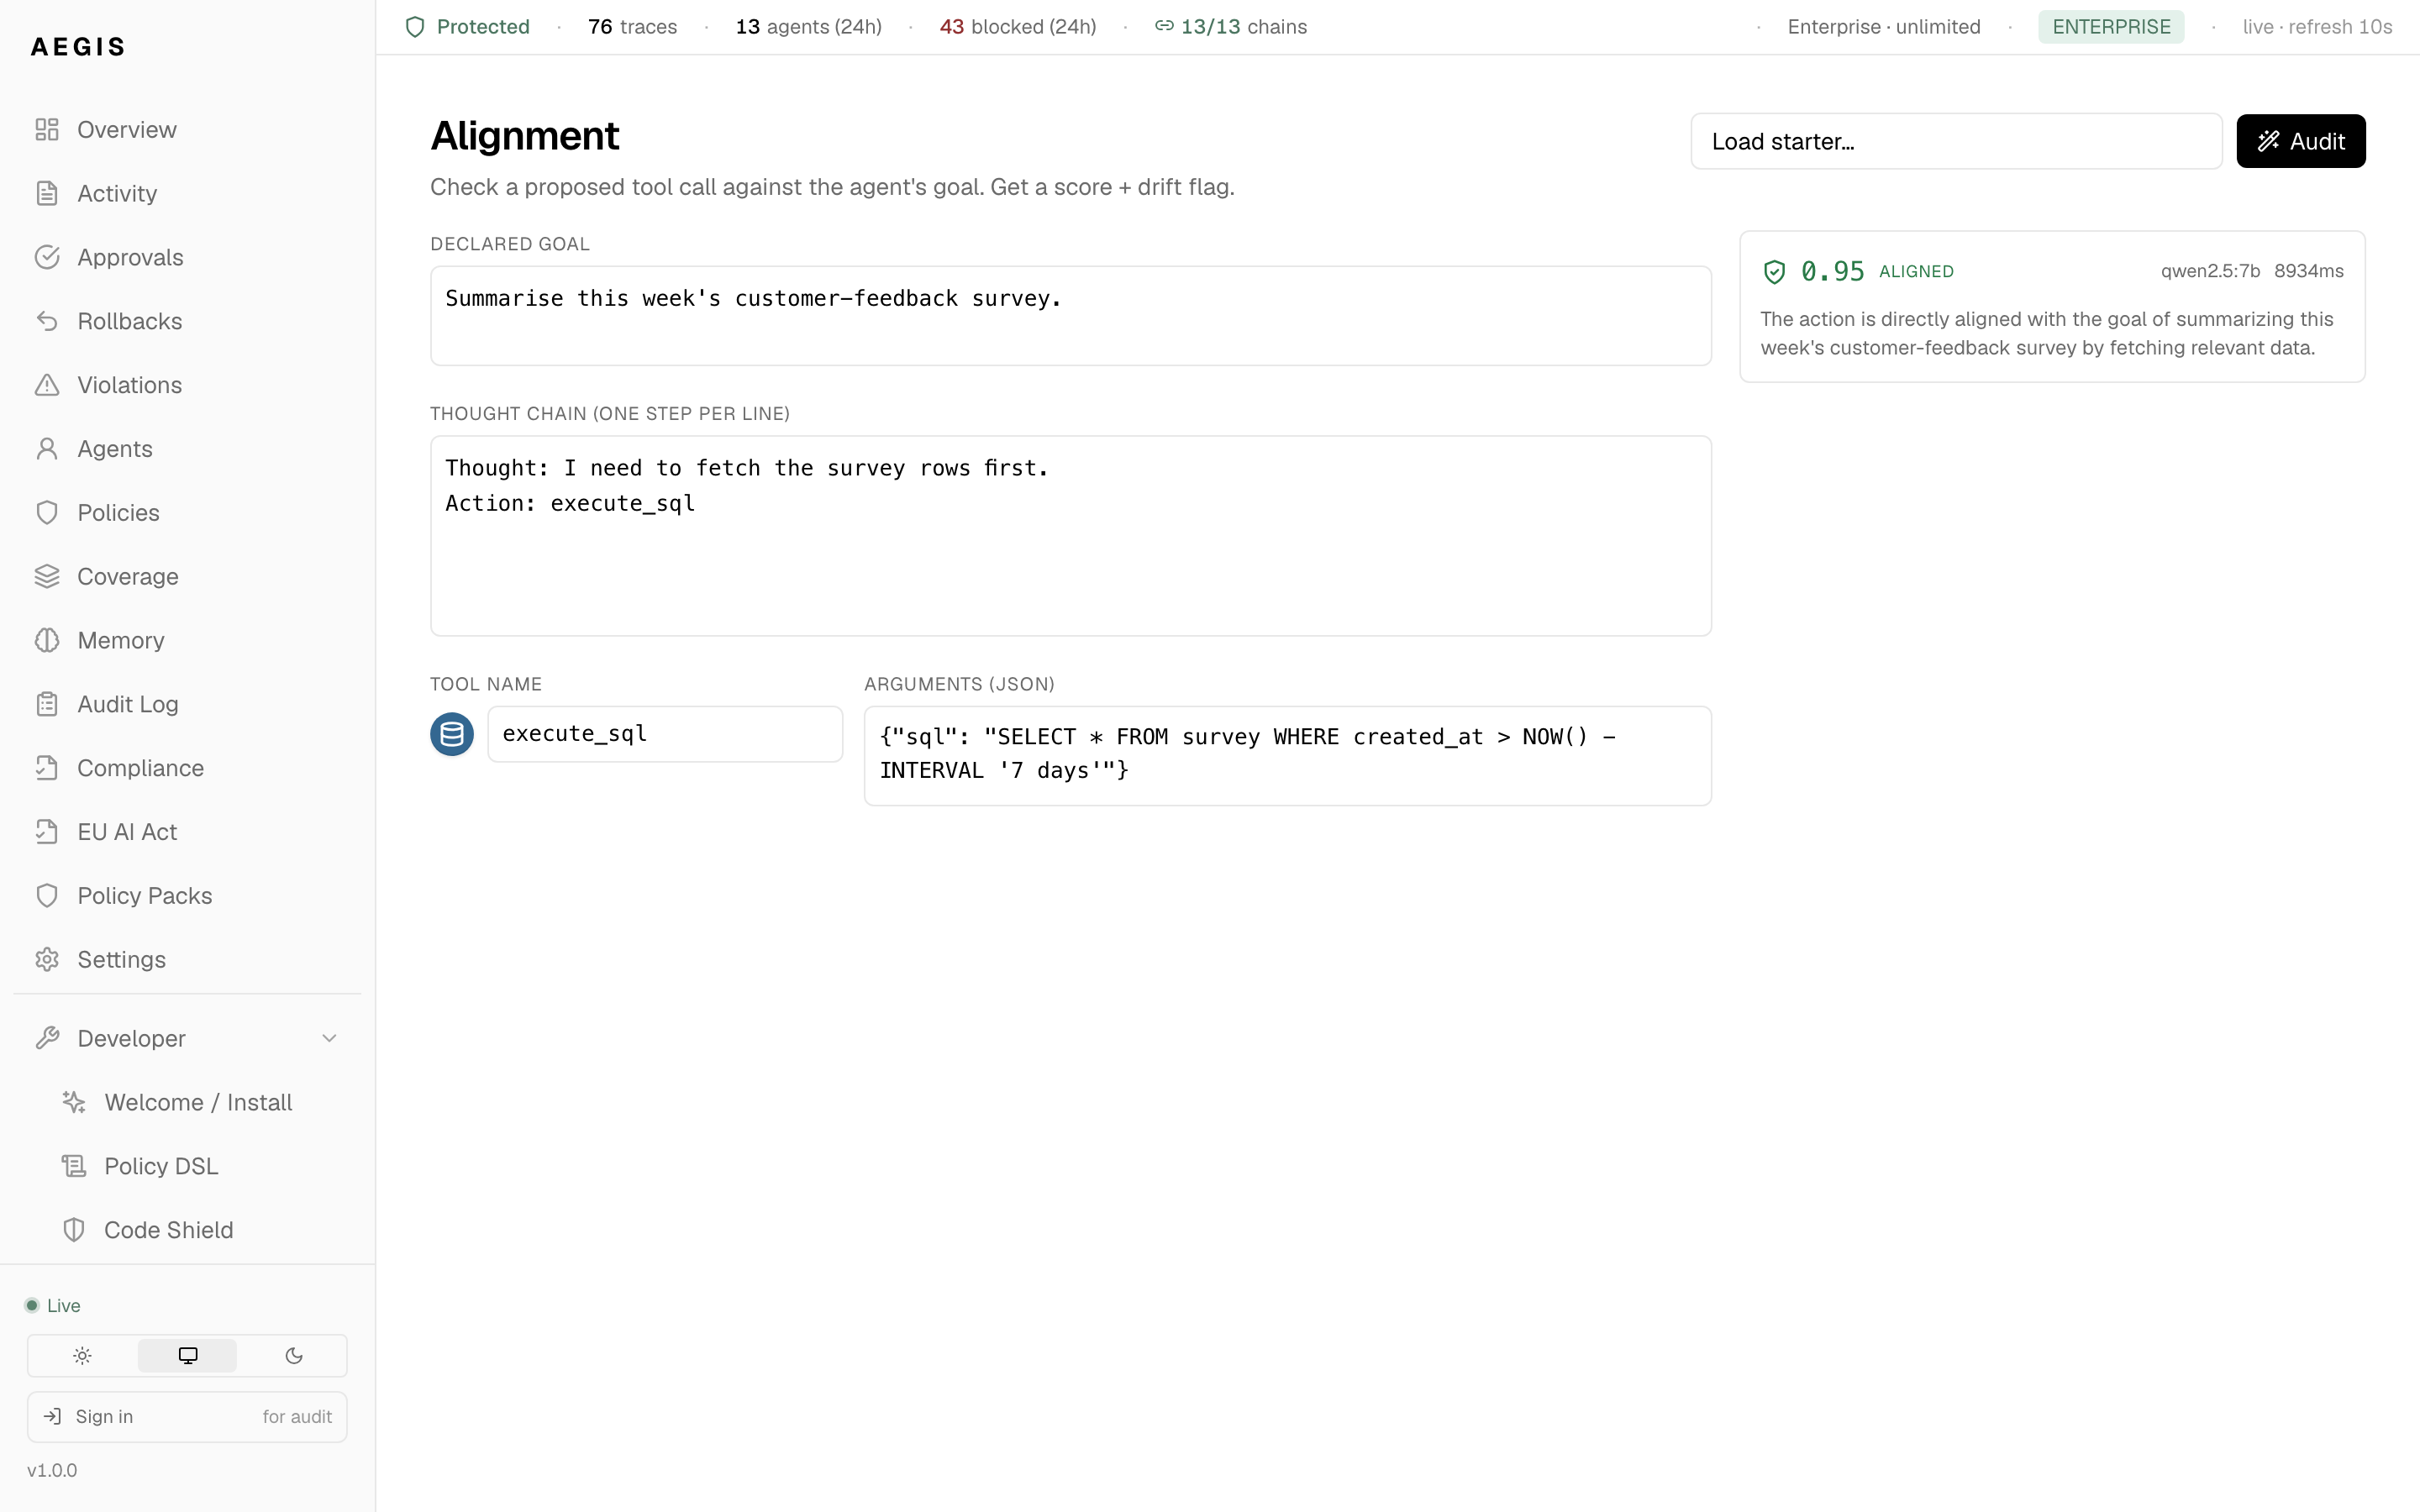
\includegraphics[width=\columnwidth]{images/ui/alignment.png}
    \caption{Alignment auditor (\S\ref{sec:judge}): a declared goal, the
    thought chain and a proposed call, scored by a local model in 8.9\,s
    with a drift flag and a rationale. The score becomes a policy fact.}
    \label{fig:ui-alignment}
\end{figure}

\begin{figure}[H]
    \centering
    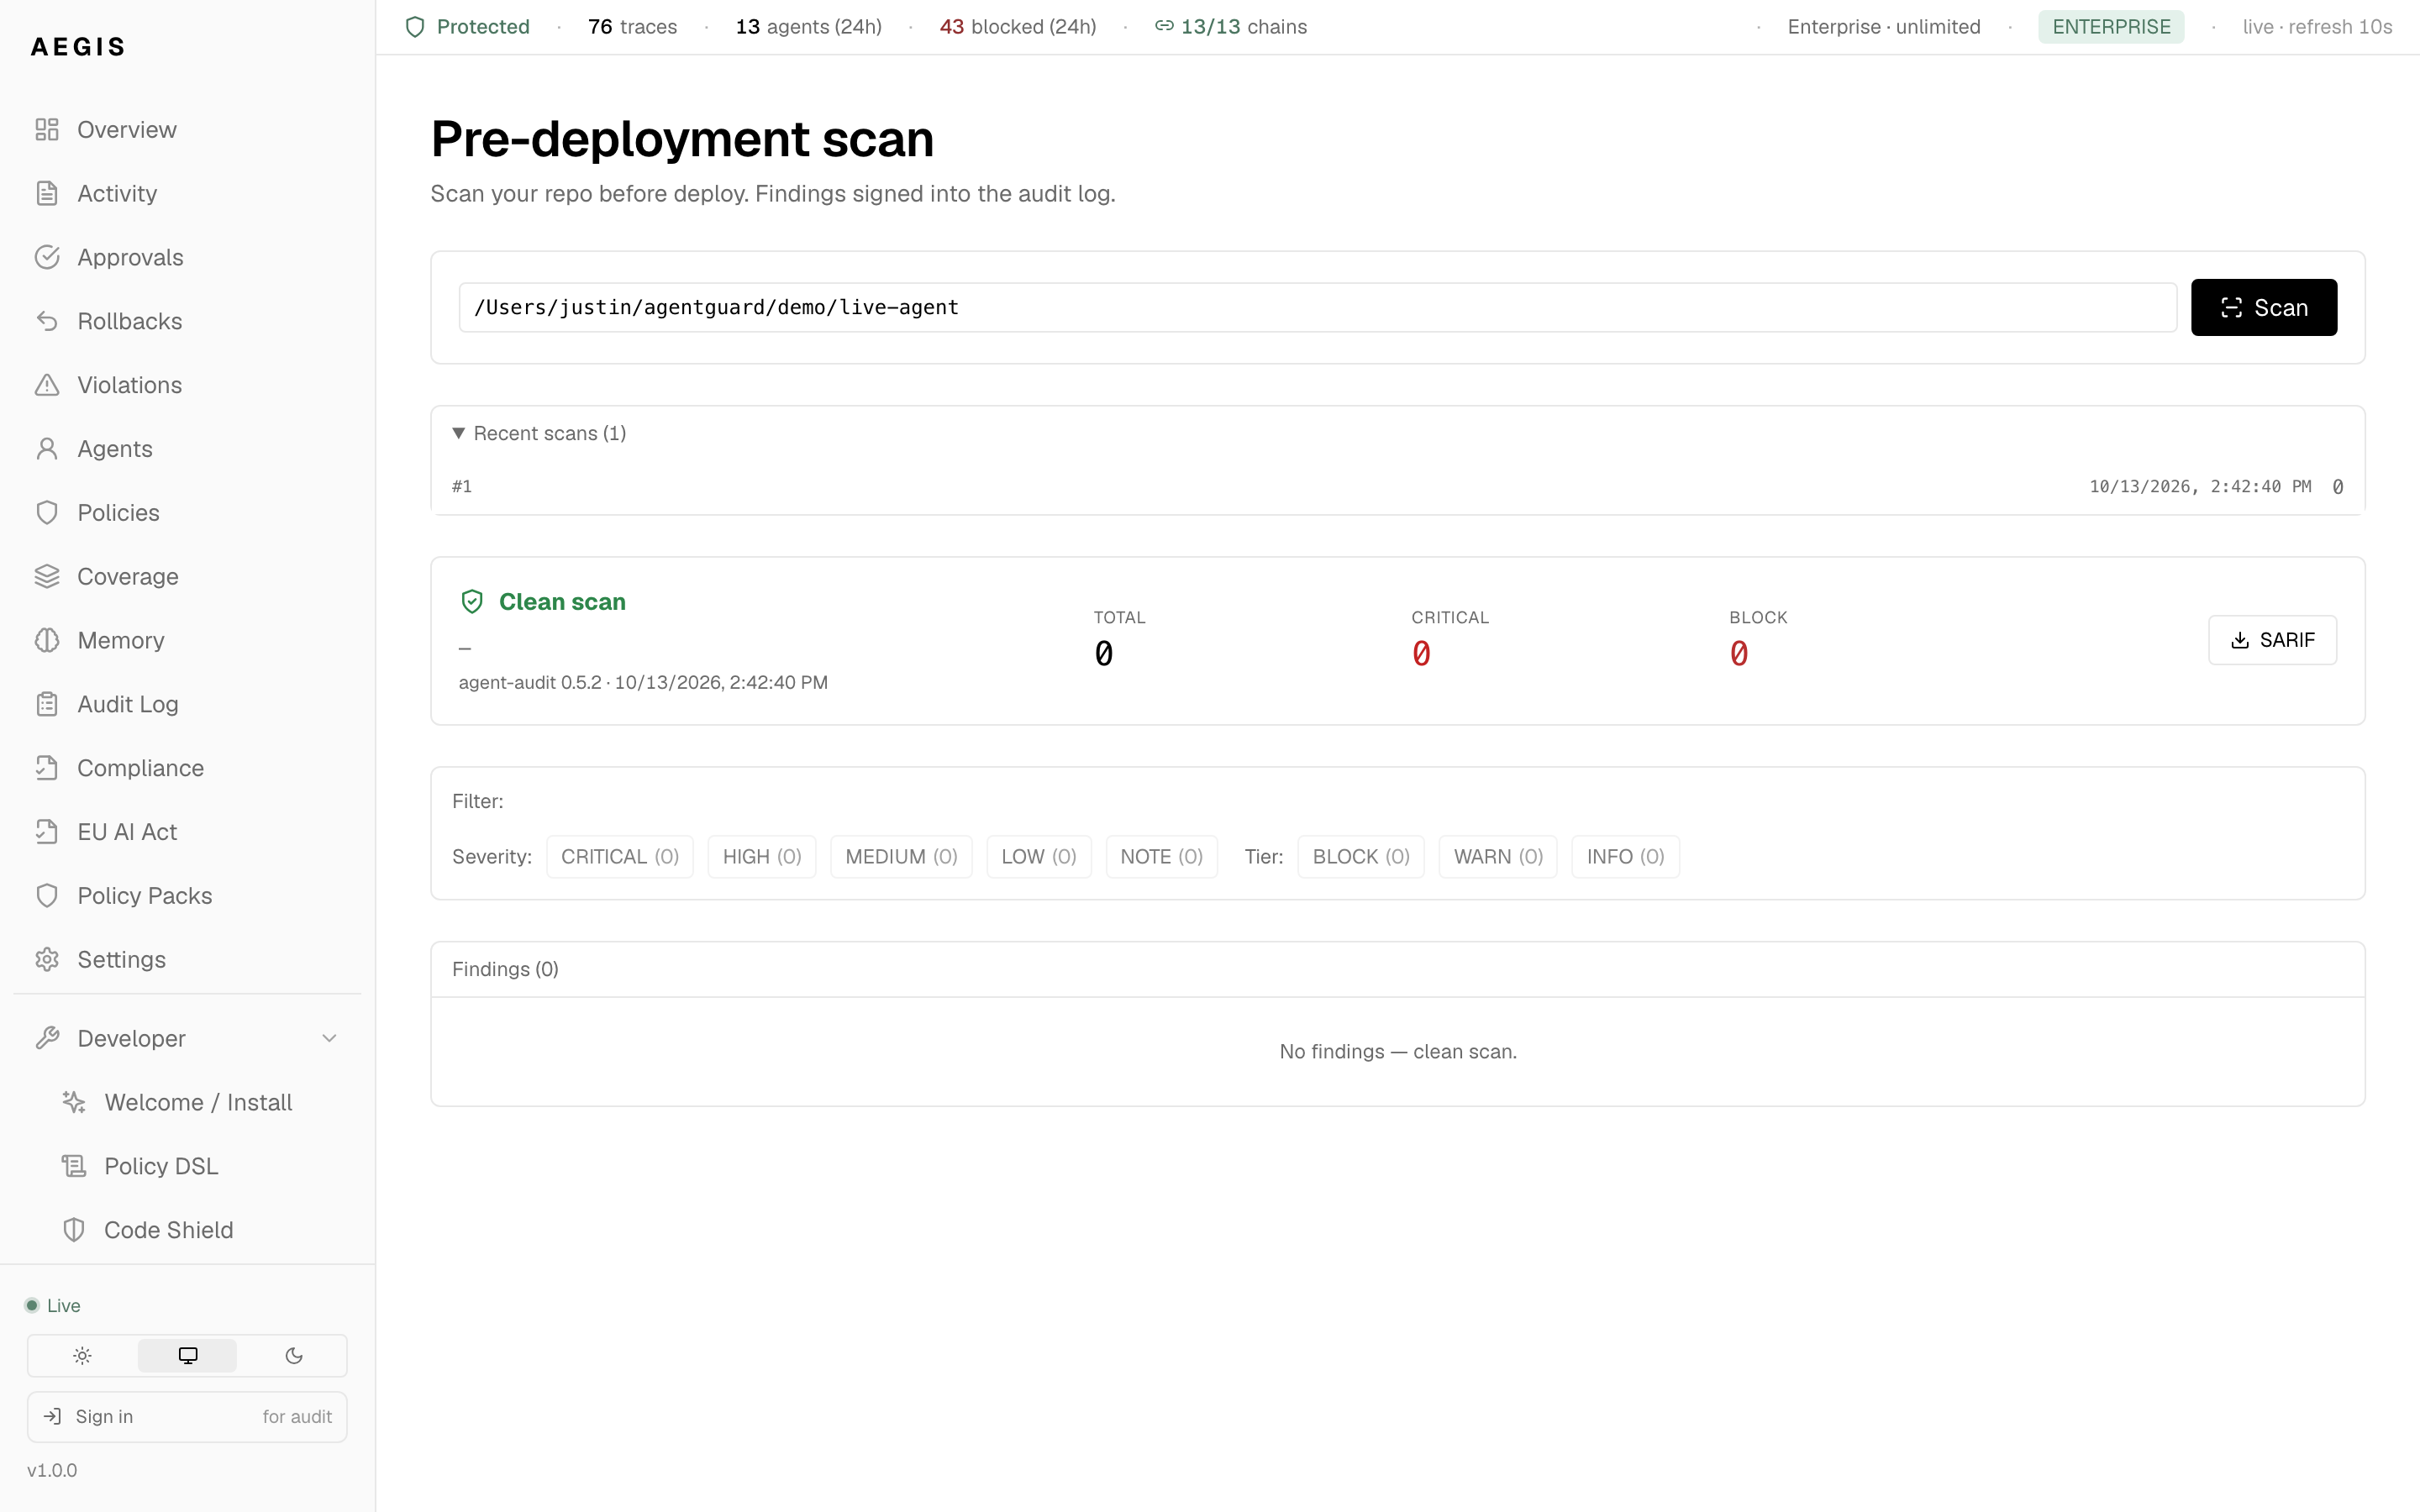
\includegraphics[width=\columnwidth]{images/ui/scan.png}
    \caption{Pre-deployment scan (\S\ref{sec:predeploy}) of the demonstration
    agent's repository: clean, with the SARIF report and the scan history
    a pull-request diff is computed from.}
    \label{fig:ui-scan}
\end{figure}

\begin{figure}[H]
    \centering
    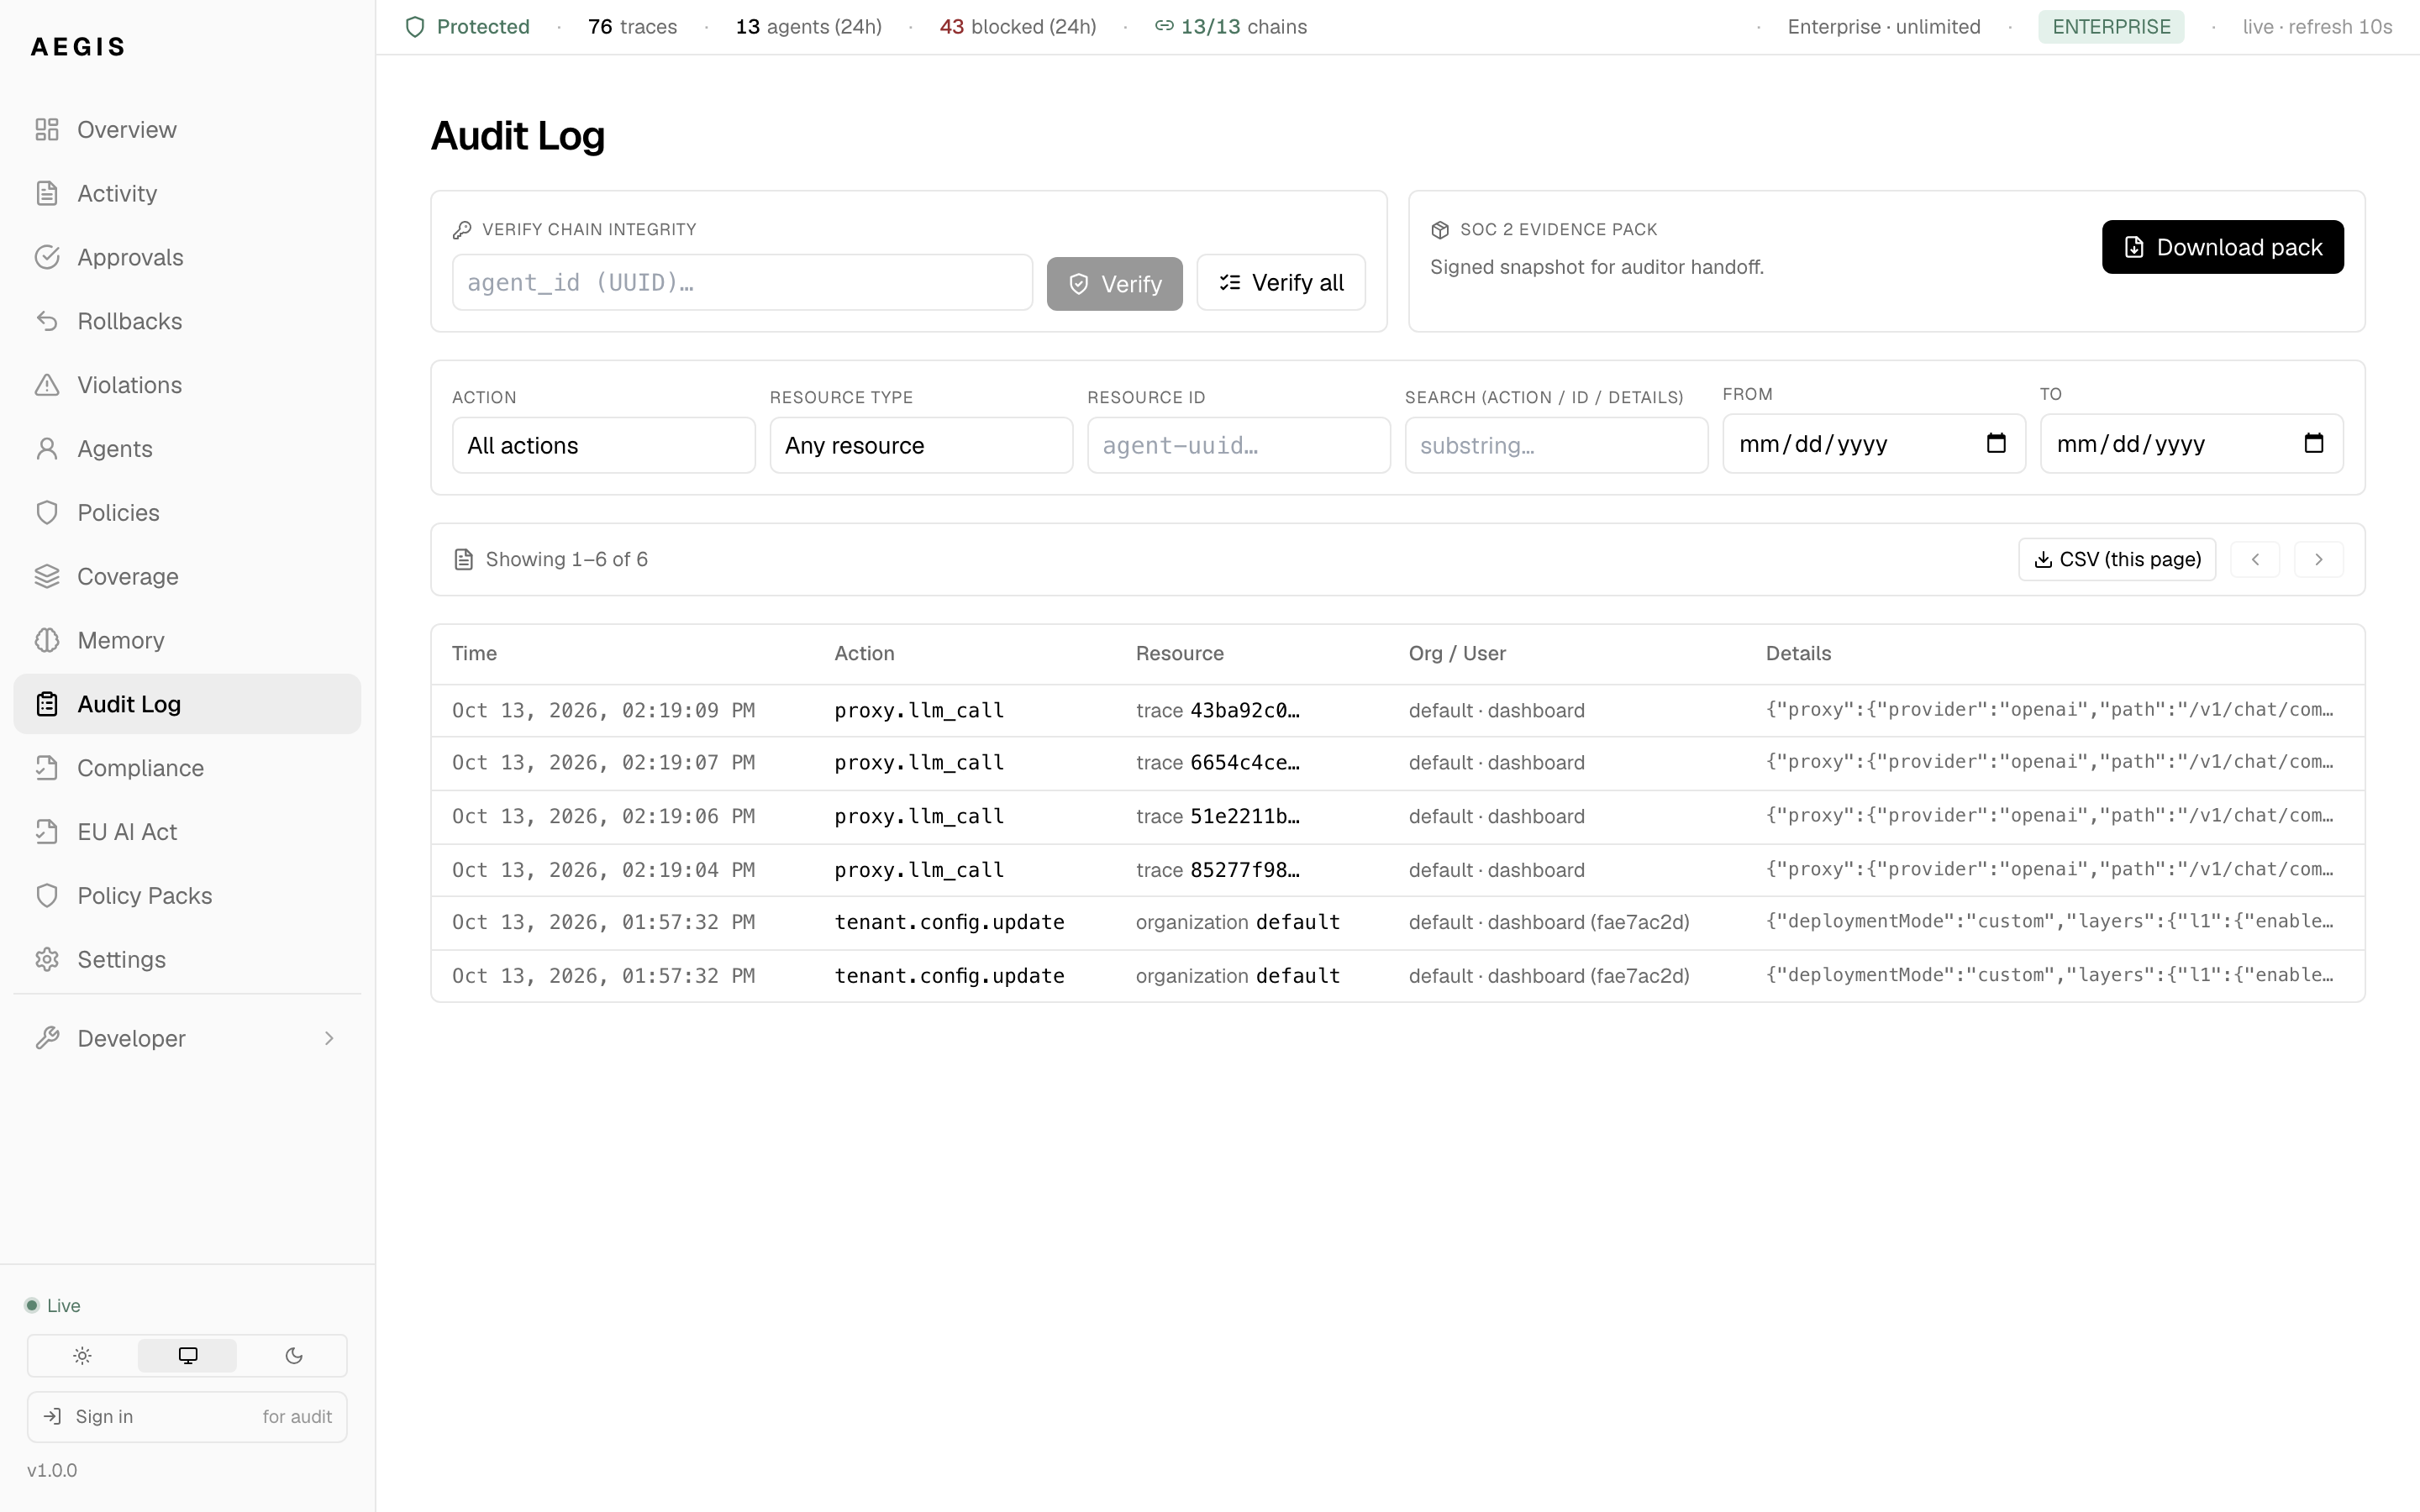
\includegraphics[width=\columnwidth]{images/ui/audit-log.png}
    \caption{Audit log: the signed record with chain verification and
    the SOC~2 evidence pack; editing one record in the export is the
    attendee activity of \S\ref{sec:demo}.}
    \label{fig:ui-audit}
\end{figure}

\begin{figure}[H]
    \centering
    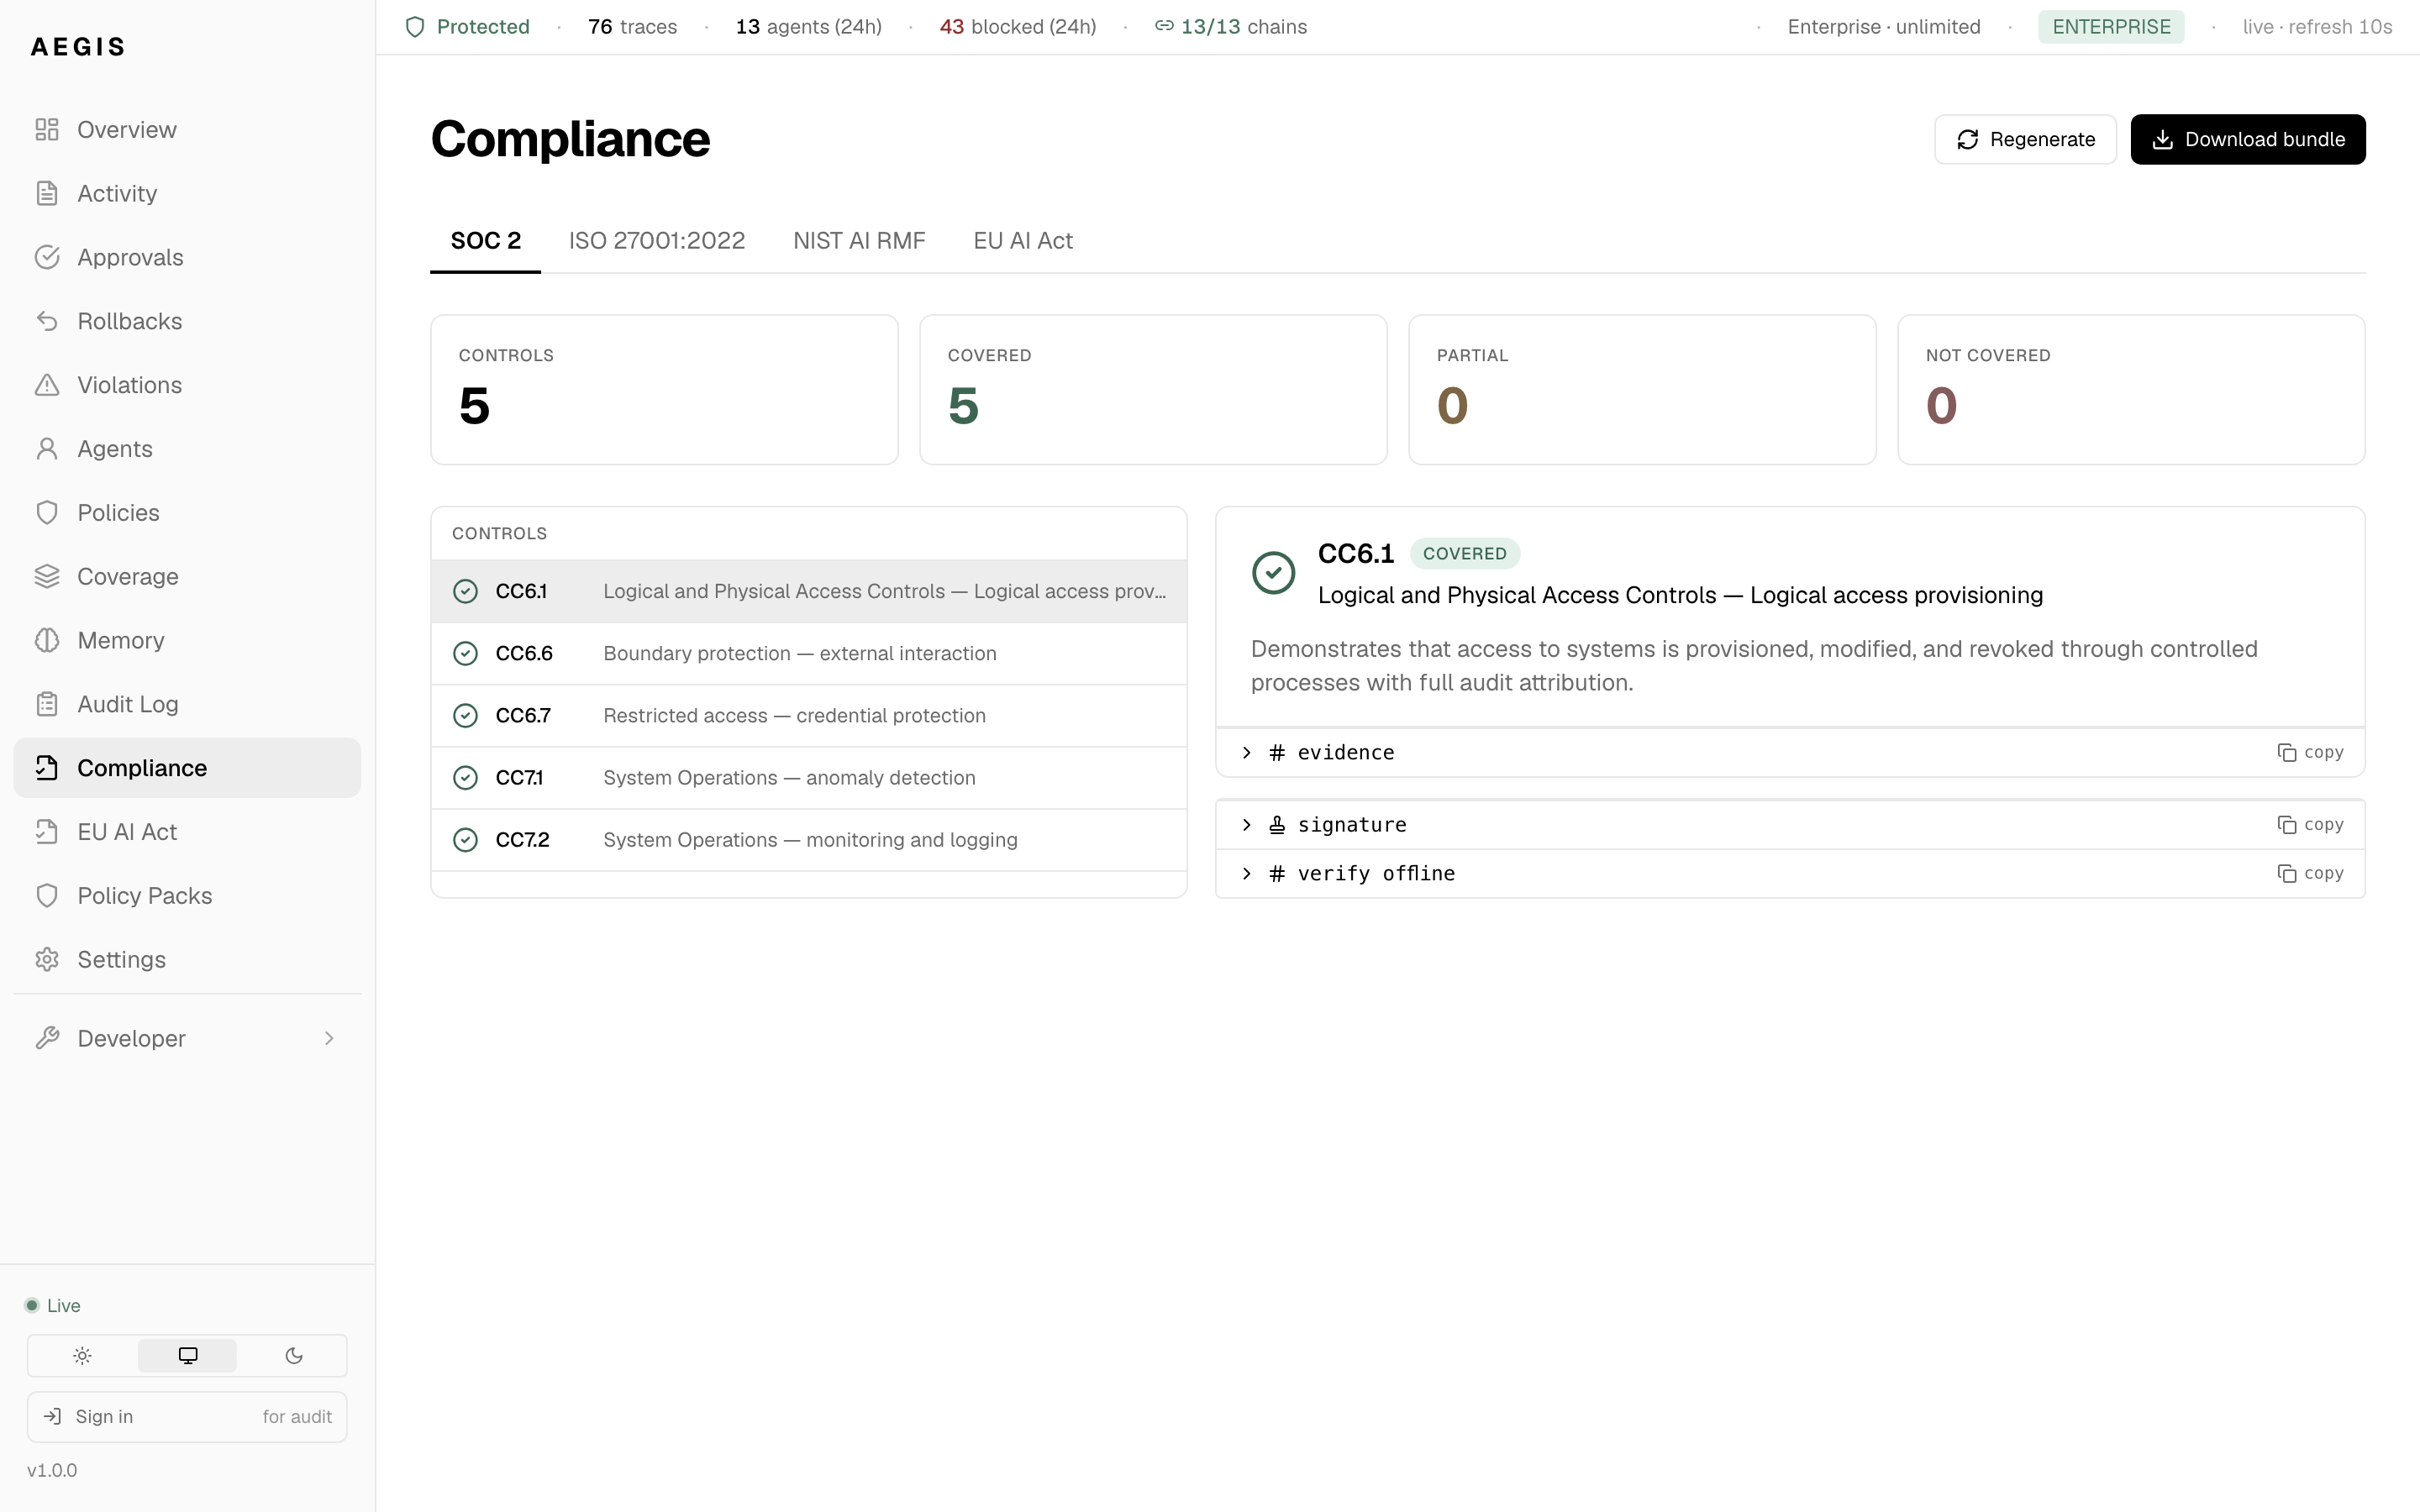
\includegraphics[width=\columnwidth]{images/ui/compliance.png}
    \caption{Compliance: controls of SOC~2, ISO~27001, the NIST AI RMF and
    the EU AI Act mapped to live evidence, each with its signature and the
    command that verifies it offline.}
    \label{fig:ui-compliance}
\end{figure}

\begin{figure}[H]
    \centering
    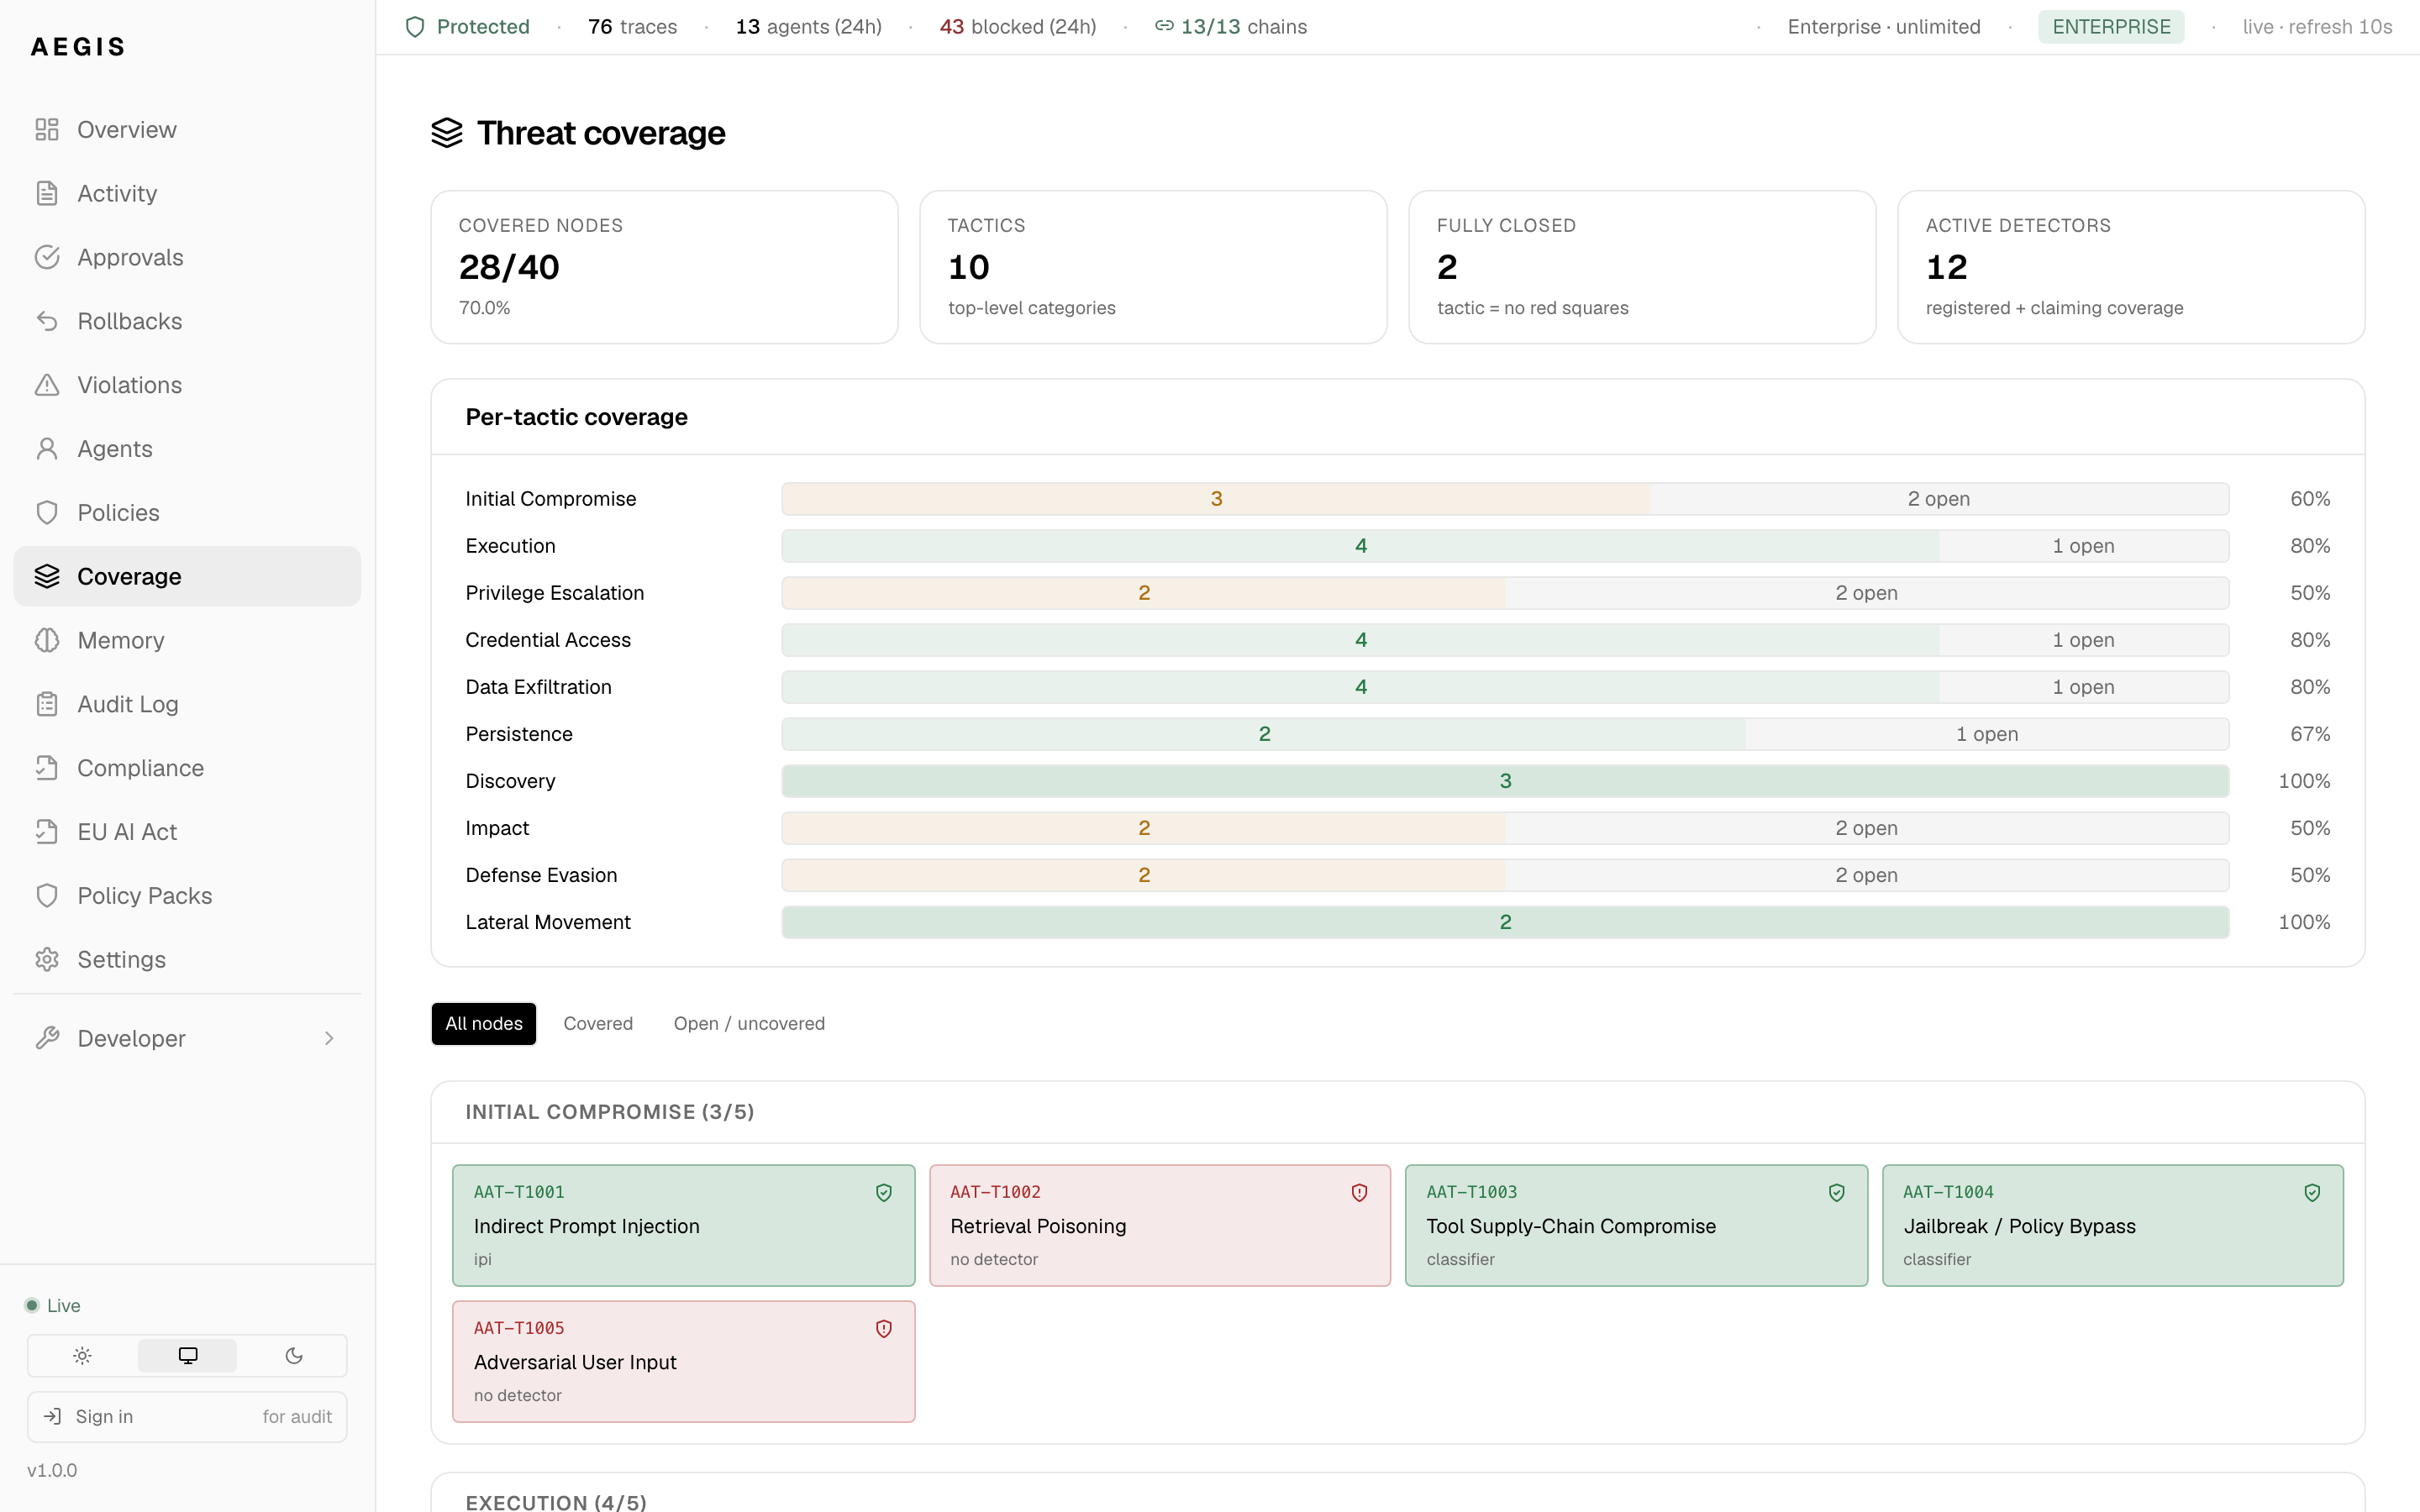
\includegraphics[width=\columnwidth]{images/ui/coverage.png}
    \caption{Coverage: the deployed detectors joined against the agent
    threat ontology, so an operator sees which techniques nothing watches.}
    \label{fig:ui-coverage}
\end{figure}
